




%
%
\chapter{Introduction}\label{ch_introduction}



%
%
\section{Scope of the Thesis}

\textit{Machine learning}, defined by Arthur Samuel in $1959$ as ``a field of study that gives computers the ability to learn without being explicitly programmed'', has gained in popularity and become an active research field in computer science during the last few decades.
Machine learning not only produces intelligent systems that generalize well from previously observed examples, but is also firmly rooted in statistical learning theory that establishes the conditions guaranteeing good generalization \citep{Vapnik98statistical,Vapnik99an}.
Machine learning appears in many real world applications, to name but a few, ranking web page in internet search \citep{Richardson06beyond}, spam filtering in email \citep{Goodman06online}, recommender systems for online shopping \citep{Bell07lessons}, and image and speech recognitions \citep{Bengio09learning}.
With the increasing availability of large scale datasets, machine learning is expected to play an indispensable role in many research fields \citep{Fan13mining}.

\textit{Supervised learning}, an important paradigm in machine learning, is usually defined as learning a function that is capable of predicting the best value for an output variable given an input variable.
The function is learned by exploring a set of observed input/output pairs known as training examples.
In the classical supervised learning setting, there is only one variable to be predicted.
This is called \textit{single-label classification} if the output variable is discrete, or \textit{regression} if the output variable is continuous.
Many single-label classification models have been designed and applied in practice, for example, the Perceptron \citep{Rosenblatt58}, Logistic Regression \citep{Chen99}, and Support Vector Machines \citep{Cortes95support}.

\textit{Multilabel classification} is a natural extension to single-label classification by defining multiple interdependent output variables associated with each input.
These type of problems are prevalent in everyday life.
For example, a movie can be classified as ``sci-fi'', ``thriller'' and ``crime''; a news article can be categorized as ``science'', ``drug discovery'' and ``genomics''; a gene can be associated with multiple functions in genomics research; a surveillance photo can be tagged with ``car'', ``building'' and ``road''. 
When multiple output variables are treated as a ``flat'' vector, the problem is often called \textit{flat multilabel classification}.
Flat multilabel classification is one branch of multilabel classification that has drawn increasing amount of interest from the machine learning community \citep{Tsoumakas07multi,Tsoumakas10mining}.
As multiple output variables can be ``on'' and ``off'' simultaneously, various flat multilabel classification algorithms have been developed that aim to explore the correlation between multiple output variables in order to make accurate predictions.
In particular, \citet{Tsoumakas07multi} summarized the established flat multilabel classification algorithms into two categories: problem transformation approaches \citep{Zhang05a,Read09classifier,Cheng09combining} and algorithm adaptation approaches \citep{Schapire99improved,Bian12corrlog}

%Flat multilabel classification has been tackled by many algorithms that aim to explore the correlation or the dependency between multiple output variables in order to make better prediction \citep{Schapire99improved,Zhang05a,Read09classifier,Cheng09combining,Bian12corrlog}.

There exists another line of research in multilabel classification known as \textit{structured output prediction} where a complex structure (\textit{output graph}) is defined on multiple output variables to model dependencies in a more comprehensive way.
\textit{Hierarchical classification} is one type of structured output prediction in which the prediction needs to be reconciled along a pre-established hierarchical structure \citep{Silla11a}.
Hierarchical classification is usually applied to the problem with different level of granularity. 
The hierarchy can be either a rooted tree such as in the document classification problem \citep{Hao07hierarchicaly,Li07hierarchical,Rousu06}, or a directed acyclic graph (\daggraph) with parent-children relationships such as in the gene function prediction problem \citep{Barutcuoglu06hierarchical}.
There exists a large body of work on hierarchical classification from the early approaches which use the hierarchical structure heuristically for preprocessing or post-processing \citep{Koller97hierarchically,Dumais00Hierarchical,Liu05support,DeCoro07bayesian} to the recent approaches which encodes the structure into learning \citep{Cai04hierarchical,Cesabianchi05incremental,Rousu06,Gopal12bayesian}.

\textit{Graph labeling} is another type of structured output prediction in which the output graph often takes a more general form and does not require the concept of ``level'' compared to hierarchical classification.
The approach can be applied to a wider range of problems, for example, speech tagging with sequence structure \citep{collins02a}, and action recognition with Markov network structure \citep{Wang11hidden}. 
The graph labeling approach often directly incorporates the output graph into learning and exploits the correlation between labels to improve classification performance \citep{collins02a,lafferty01,taskar02,Taskar04max,THJA04,Rousu07}.
For graph labeling or structured output learning in general, one inherited problem is the output graph is assumed to be observed \textit{apriori}.
However, this cannot be taken for granted since the proper dependency structure for the output variables is either hidden or difficult to retrieve in many applications \citep{Chickering94learning}.

Figure~\ref{multilabel_taxonomy} illustrates the taxonomy of multilabel classification.
However it is worth pointing out that there is no clear line drawn between different categories.
In particular, some hierarchical classification algorithms can also belong to the graph labeling category, for example, those developed by \citet{THJA04,Rousu06}.
As we focus on graph labeling in structured output prediction, we will explicitly use ``structured output prediction'' to refer to ``graph labeling'' throughout the thesis.

\begin{figure}
\begin{center}
	\centering
	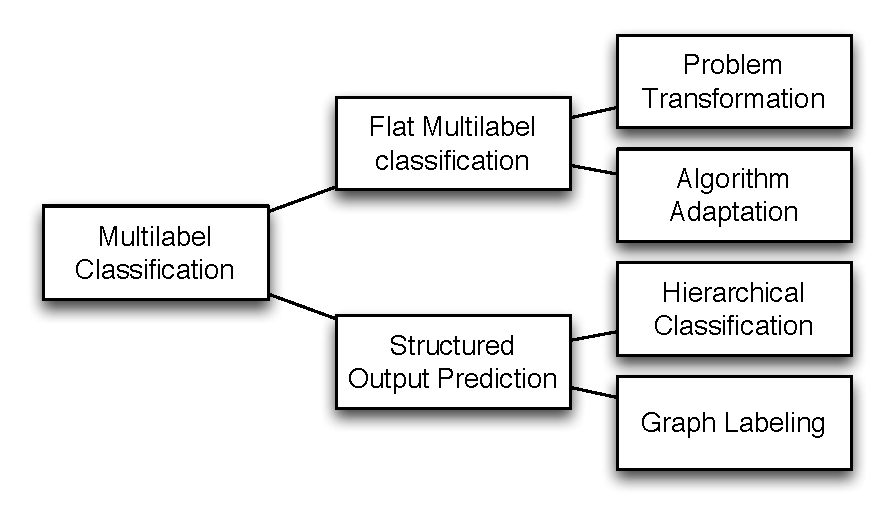
\includegraphics[width=10.5cm]{./taxonomy.pdf}
	\caption{The taxonomy of multilabel classification.}
	\label{multilabel_taxonomy}
\end{center}
\end{figure}

In this thesis, we extend the applicability of structured output learning by developing new learning algorithms and applying them to real world multilabel classification problems.
In addition, we work on the problem of structured output learning when the output dependency structure is not observed.
The models thus created are not restricted to the availability of the output graph and can therefore be applied to a wider range of multilabel classification problems.
We also investigate the efficiency and the scalability of the inference algorithms in the proposed structured output learning models.
Finally, we study the theoretic aspect of the proposed methods.
The research questions can be summarized as follows.
\begin{itemize}
\item Should we tackle the multilabel classification problems with structured output learning rather than using flat multilabel classification approaches?
\item How to apply structured output learning to the multilabel classification problems when the output graph is not observed?
\item Can we provide any theory to explain the behavior of the proposed structured output learning models and to guarantee the performance?
\item Can we efficiently solve the inference problems of the proposed structured output learning models?
\end{itemize}



%
%
\section{Contributions and Organization}

The contributions of the thesis are several statistical learning algorithms that widen the applicability of structured output learning.
The thesis starts by reviewing several lines of research in classification learning.
The first contribution is to develop a new structured output learning algorithm for the multilabel classification problem with an observed output graph.
The proposed algorithm can predict a directed acyclic graph (\daggraph) from an observed underlying network which best responses to an input.
The algorithm has applied to network response prediction within the context of social network analysis.
For the general multilabel classification problem in which the output graph is not known \textit{apriori}, we develop several new algorithms that combine a set of structured output learners built on a collection of random output graphs.
In addition, we develop a joint learning and inference framework that is based on Max-Margin learning on a random sample of spanning trees.
Thus, the proposed methods are not constrained by the availability of the output graphs.
Moreover, we provide the theoretic studies which not only explain the intuition behind the formalisms but also guarantee the generalization error of the proposed models.

The remaining part of this thesis is structured as follows.
Chapter~\ref{ch_rlc} gives the background information to the learning problem in terms of classification, covering the basic concepts in classification learning including regularized risk minimization in Section~\ref{sc_rrm}, single-label classification in Section~\ref{sc_slc}, and ensemble learning in Section~\ref{sc_em}.
Chapter~\ref{ch_fmlc} introduces the multilabel classification problem which is the core problem under study in this thesis.
The chapter also describes the flat multilabel classification approach which is a standard treatment for the multilabel classification problem.
Chapter~\ref{ch_sop} and Chapter~\ref{ch_sopw} present the main contributions of the thesis.
In particular, Chapter~\ref{ch_sop} presents the structured output learning models developed for the multilabel classification problem with an observed output graph.
The methods presented extend the flat multilabel classification approaches described in the previous chapter.
Chapter~\ref{ch_sopw} discusses several learning methods developed for structured output learning when the output dependency structure is not observed.
Chapter~\ref{ch_implementation} describes the implementation details of the developed models.
Chapter~\ref{ch_conclusion} concludes the thesis and details the future research directions.

The thesis presents the idea and the background of the proposed structured output learning methods.
The formalisms of the proposed methods are also briefly explained.
The technical details can be found in the original research articles in the latter part of the thesis.
The notation and the presentation of some of the proposed models are slightly improved in order to incorporate the methods into a unified framework.
Empirical evaluations of the proposed models are not repeated, rather, they can be found from the original research articles in the latter part of the thesis.



%------------------------------------------------
%
%
%
%------------------------------------------------
\chapter{Regularized Learning for Classification} \label{ch_rlc}



%------------------------------------------------
%
%------------------------------------------------
\section{Regularized Risk Minimization}\label{sc_rrm}

In this section, the author will introduce two fundamental concepts in statistical machine learning, known as \textit{empirical risk minimization} \citep{Vapnik92principles} and \textit{regularization} \citep{Evgeniou99a} which create most learning algorithms presented in the following part of this thesis.

\subsection{Empirical Risk Minimization}\label{sc_erm}

We assume that two random variables $\vx\in\vXcal$ and $y\in\Ycal$ are jointly distributed according to some fixed but unknown probability distribution $P(\vx,y)$ over domain $\vXcal\times\Ycal$, where $\vXcal$ is an input (instance) space and $\Ycal$ is an output (label) space.
The definition of the output space $\Ycal$ will decide the type of the learning problem,
for example, 
multiclass classification by setting $\Ycal=\{1,\cdots,K\}$,
regression by setting $\Ycal=\RR$ where $\RR$ is a set of real numbers,
binary classification by setting $\Ycal=\{-1,+1\}$, 
and multilabel binary classification by setting $\Ycal = \{-1,+1\}^k$.
In addition, we are provided with paired examples $(\vx,y)\in\vXcal\times\Ycal$ which are generated by sampling according to the distribution $P(\vx,y)$.
A \textit{hypothesis class} $\Hcal$ is a set of functions that a learning algorithm is allowed to search against.
The goal of statistical learning is to provide an \textit{estimator} $f\in\Hcal:\vXcal\rightarrow\Ycal$ which predicts the best value of an output $y$ given an input $\vx$.

We use \textit{loss function} $\Lcal(y,f(\vx)):\Ycal\times\Ycal\rightarrow\RR^+$ to measure the goodness of an estimator, which is a monotonic bounded function between a true value $y$ and an estimated value $f(\vx)$.
There are many ways of defining the loss function including, for example,
\textit{Hinge Loss} in Support Vector Machines \citep{Cortes95support}
\begin{align}
	\Lcal_{hinge}(y,f(\vx)) = \maximize (0,1-y f(\vx)),\, \Ycal=[-1,+1], \label{hinge_loss}
\end{align}
\textit{$0/1$ Loss} in structured \svm\ \citep{THJA04}
\begin{align}
	\Lcal_{0/1}(y,f(\vx)) = \ind{y=f(\vx)},\, \Ycal = \{-1,+1\}^k, \label{one_loss}
\end{align}
\textit{Squared Loss} in Ridge Regression \citep{Hoerl00ridge}
\begin{align*}
	\Lcal_{squared}(y,f(\vx)) = (y-f(\vx))^2,\, \Ycal=\RR,
\end{align*}
\textit{Exponential Loss} in \adaboost\ \citep{Schapire99improved}
\begin{align}
	\Lcal_{exp}(y,f(\vx)) = \exp(-y f(\vx)),\, \Ycal=\RR, \label{exp_loss}
\end{align}
and \textit{Logistic Loss} in Logistic Regression \citep{Chen99}
\begin{align}
	\Lcal_{log}(y,f(\vx)) = \log(1+\exp(-y f(\vx))),\, \Ycal=[-1,+1]. \label{log_loss}
\end{align}
We will study loss functions with corresponding learning algorithms in detail in the following part of this thesis.

The \textit{true risk} of an estimator $f$ over all examples from a domain $\vXcal\times\Ycal$ is then defined as
\begin{align}
	\Rcal(f) = \int_{(\vx,y)\in\vXcal\times\vYcal}\Lcal(y,f(\vx))P(\vx,y)\,d_{\vx}d_{y} \label{true_risk}.
\end{align}
As a result, the learning algorithm should search for an estimator $f\in\Hcal$ which minimizes the true risk (\ref{true_risk}).
However, it is impossible to compute the true risk (\ref{true_risk}) directly, as the distribution $P(\vx,y)$ is unknown.
Instead we are given a random sample of $m$ examples, denoted by $S=\{(\vx_1,y_1),\cdots,(\vx_m,y_m)\}$, called \textit{training data}.
The \textit{Empirical risk} of an estimator $f\in\Hcal$ is defined as the average error made by the estimator on a training data $S$ of finite size
\begin{align}
	\Rcal_{emp}(f) = \frac{1}{m}\sum_{i=1}^{m}\Lcal(y_i,f(\vx_i)) \label{empirical_risk}.
\end{align}
This suggests that the learning algorithm should search for an estimator to minimize the empirical risk (\ref{empirical_risk}), which is called {empirical risk minimization} \citep{Vapnik92principles} in machine learning.

\subsection{Regularized Learning}\label{sc_rl}

The empirical risk minimization strategy is ill-posed as it will provide infinite number of estimators with the same empirical risk on the same training data.
Besides, it quite often leads to \textit{overfitting}, in particular when the dimensionality of the feature space is high and the number of training examples is relatively small.
That is, the underlying true distribution $P(\vx,y)$ is difficult to estimate based on a finite sample of training examples.
As a result, the estimator will generalize poorly on unseen test examples.
Regularization theory \citep{Evgeniou99a,Evgeniou02regularization} provides a framework to tackle those two problems.
In particular, it suggests to minimize 
 \begin{align}
	\Jcal(f) = \Rcal_{emp}(f) + \lambda\Omega(f), \label{rl}
\end{align}
where $\Omega(f)$ is a regularization function that controls the complexity of the estimator by penalizing the norm of the feature weight vector, $\lambda$ is a positive parameter that controls the relative weight between the empirical risk term and the regularization term.

For the linear function class, there are several ways to define the regularization term including, for example, $L_1$-norm and $L_2$-norm regularization.
$L_2$-norm regularization, defined by 
\begin{align}
	\Omega_{L_2}(f) = ||\vw||_2=\left(\sum_{i=1}^d|\vw[i]|^2\right)^{\frac{1}{2}}, \label{l2_norm}
\end{align} 
controls the complexity of the estimator $f$ and provides a smooth solution.
It has been applied in, for example, Ridge Regression \citep{Hoerl00ridge}, Logistic Regression \citep{Chen00}, and Support Vector Machines \citep{Cortes95support}.
On the other hand, $L_1$-norm regularization, defined by
\begin{align*}
	\Omega_{L_1}(f) = ||\vw||_1=\sum_{i=1}^d|\vw[i]|,
\end{align*}
provides sparse parameter estimations such that we obtain a high dimensional feature weight vector with many zero entries.
This is an attractive property as \textit{feature selection} is incorporated into the learning process and the resulting model is usually easy to interpret.
The $L_1$-norm regularization has been applied in, for example, \lasso\ \citep{Tibshirani94regression}.
Many other regularization techniques have been widely studied, for example, $L_{1,2}$-norm regularization \citep{Argyriou07multitask}, and elastic net regularization \citep{Zou05regularizationa}.


%------------------------------------------------
%
%------------------------------------------------
\section{Single-Label Classification}\label{sc_slc}

In this section, the author will introduce the basic classification problem known as {single-label classification}, and explain two prominent algorithms in this area, namely Logistic Regression and Support Vector Machines.
Optimization techniques and the latest advances of these two algorithms will also be briefly discussed.
The goal is to provide background information that is necessary to understand the algorithms presented in the latter part of this thesis. 



%
%
\subsection{Preliminaries}\label{sc_slc_pn}

In this section, we focus on the standard supervised learning problem also known as \textit{binary classification}, by explicitly assuming the output space $\Ycal=\{-1,+1\}$.
Additionally, we assume a feature map $\varphib:\vXcal\rightarrow\vFcal$, which embeds an input into some high dimensional feature space $\vFcal=\RR^d$.
In particular, $\varphib(\vx)$ is a vector of real values in $d$ dimensions.
%Given a training set of $m$ training examples $\Scal=\{(\vx_1,y_1),\cdots,(\vx_m,y_m)\}$, the goal is to learn a mapping function $f\in\Hcal:\vXcal\rightarrow\Ycal$ from a {hypothesis class} $\Hcal$ that maps an input $\vx\in\vXcal$ to an output $y\in\Ycal$. 
We consider the hypothesis class to be a set of \textit{linear classifiers} that is parameterized by a weight vector $\vw$ and a bias term $b$ defined as
\begin{align}
	f(\vx;\vw,b) = \ip{\vw}{\varphib(\vx)} + b, \label{linearclassifier}
\end{align}
where $\ip{\cdot\,}{\cdot\,}$ denotes the inner product of two vectors
\begin{align*}
	\ip{\vw}{\varphib(\vx)} = \sum_{i=1}^{d}\vw[i]\,\varphib(\vx)[i].
\end{align*}
For any $1\le\rho\in\RR$, the {$L_{\rho}$-norm of a vector $\vw$ is defined as
\begin{align*}
	\norm{\vw}_{\rho} = \left(\sum_{i=1}^{d}|\vw[i]|^{\rho}\right)^{\frac{1}{\rho}}.
\end{align*}
For the convenience of presentation, we will explicitly use $||\vw||$ to refer to the $L_2$-norm of $\vw$ throughout the thesis.



%
%
\iffalse
\subsection{Perceptron}\label{sc_perceptron}

The Perceptron developed in \citep{Rosenblatt58,Rosenblatt62} is a linear classifiers parameterized by a weight vector $\vw$ and a bias term $b$. 
The decision boundary, given by 
\begin{align*}
	f(\vx;\vw,b) = \ip{\vw}{\varphib(\vx)} + b =0,
\end{align*}
will separate the data into two classes.
The parameter $\vw$ and $b$ is obtained by minimizing the distance of misclassified training examples to the decision boundary.
Assume data point $(\vx_i,y_i)$ is misclassified, the signed geometric distance from $\vx_i$ to decision boundary can be computed according to
\begin{align*}
	D(\vx_i;\vw,b) = -\frac{y_i(\ip{\vw}{\varphib(\vx_i)}+b)}{\norm{\vw}}.
\end{align*}
Let $\vXcal^m$ denote the set of misclassified examples, the objective function of the Perceptron is defined as
\begin{definition}{The Perceptron Objective Function.}\label{perceptron}
	\begin{align*}
		\underset{\vw,b}{\minimize} \, D(\vw,b) = \underset{\vw,b}{\minimize} \left( -\sum_{\vx_i\in\vXcal^{m}}y_i[\ip{\vw}{\varphib(\vx_i)}+b]\right).
	\end{align*}
\end{definition}
\noindent
To optimize (Definition~\ref{perceptron}), we first assume $\vXcal^{m}$ is fixed and compute the partial gradient with respect to the parameter $\vw$ and $b$
\begin{align*}
	\frac{\partial D(\vw,b)}{\partial\vw} = -\sum_{\vx_i\in\vXcal^m}{y_i\vx_i},\quad
	\frac{\partial D(\vw,b)}{\partial b} = -\sum_{\vx_i\in\vXcal^m}{y_i}.
\end{align*}
In practice, the Perceptron uses stochastic gradient descent that iteratively processes one example from the training data at a time.
Once the example is misclassified, the algorithm adjusts the parameters according to the update rule
\begin{align*}
	\vw \leftarrow \vw + \eta y_i \vx_i, \quad b \leftarrow b + \eta y_i,
\end{align*}
where $\eta$ is the Perceptron learning rate.

\iffalse
\begin{theory}[Perceptron Convergence Theorem \citep{Block62the,Novikoff62}]\label{perceptron_theory}
	Given a sequence of training examples in pairs $\Scal=\{(\vx_1,y_1),\cdots,(\vx_m,y_m)\}$. 
	For simplicity, we consider a perceptron without bias term $b$.
	Assume $\norm{\vx_i}\le R$ for all $i\in\{1,\cdots,m\}$.
	Suppose for some $\gamma>0$ there exists a unit length vector $\norm{\hat{\vw}}=1$ such that $y_i(\ip{\hat{\vw}}{\varphib(\vx_i)})\ge\gamma$ holds for all $i$ (training data $\Scal$ is linearly separable).
	Then the number of mistakes the Perceptron algorithm makes on the sequence of training data $\Scal$ is at most ${R^2}/{\gamma^2}$.
\end{theory}
\begin{proof}
	Suppose the $k$'th mistake is made on the $i$'th training example, and current weight vector is $\vw^k$.
	In addition, we set $\vw^0=\vzero$.
	As the Perceptron makes a mistake on $(\vx_i,y_i)$, we immediately have
	\begin{align*}
		y_i\ip{\vw_k}{\varphib(\vx_i)} \le 0.
	\end{align*}
	According to update rule, we have
	\begin{align*}
		\vw^{k+1} = \vw^{k} + \rho y_i\varphib(\vx_i).
	\end{align*}
	Then, the following holds
	\begin{align*}
		\ip{\vw^{k+1}}{\hat{\vw}} = \ip{\vw^k}{\hat{\vw}} + \rho y_i\ip{\varphib(\vx_i)}{\hat{\vw}} \ge \ip{\vw^k}{\hat{\vw}} + \rho\gamma.
	\end{align*}
	Straight forward induction gives us
	\begin{align}
		\ip{\vw^{k+1}}{\hat{\vw}}\ge k\rho\gamma. \label{induction1}
	\end{align}
	We also have
	\begin{align*}
		\norm{\vw^{k+1}}^2 
		= \norm{\vw^{k} + \rho y_ix_i}^2
		= \norm{\vw^k}^2 + \rho^2\norm{\varphib(\vx_i)}^2 + 2\rho y_i\ip{\varphib(\vx_i)}{\vw^k}
		\le \norm{\vw^k}^2 + \rho^2R^2
	\end{align*}
	Straight forward induction gives us
	\begin{align}
		\norm{\vw^{k+1}}^2\le k\rho^2R^2. \label{induction2}
	\end{align}
	Together with (\ref{induction1}) and (\ref{induction2}) we have
	\begin{align*}
		k\le{R^2}/{\gamma^2}.
	\end{align*}
\end{proof}

Theory~\ref{perceptron_theory} shows that if the data are linearly separable, the perceptron algorithm will make a finite number of mistakes. 
In particular, the perceptron algorithm will iterate through the training set and will converge to a vector that well separates all training examples.
Moreover, the number of mistakes will be bounded by the minimum gap between the positive and negative examples.
That is, the algorithm converges quickly when the gap $\gamma$ is big.
We have to keep in mind that the convergence theorem does not say anything about the quality of the solution, though it is built based on the assumption that there is a ``gap'' between positive and negative examples.
\fi

It has been shown in \citep{Block62the,Novikoff62} that the Perceptron training will converge by making finite number of mistakes on the training data if the data is linearly separable.
However, the setting is less interesting for most applications where the data might not be linearly separable or it takes too long for the Perceptron to converge.
The \textit{Voted Perceptron} and the \textit{Averaged perceptron} developed by \citet{Freund99large} are extensions to the standard Perceptron.
The algorithms keep track all weight vectors encountered during training as well as their weights.
The weight can be seen as the ``survival time'' of the weight vector.
The prediction is composed by weighted majority vote.
Except for the simplicity, the Perceptron is merely a risk minimization approach.

\iffalse
\begin{align}
	y_{ts} = \sign\left({\sum_{l=1}^{k}c^l(\sign{\ip{\vw^l}{\varphib(\vx_{ts})}+b^{l}}})\right) \label{voted_perceptron_prediction}
\end{align}
using the weight vectors $\vw^l$ and the corresponding weights $c^l$ obtained during learning.
\iffalse
\textit{Voted Perceptron} developed in \citep{Freund99large} is a straight forward modification of the standard perceptron.
As described in (Algorithm~\ref{voted_perceptron}), the voted perceptron algorithm keeps track all weight vectors that appears during training phase (line~\ref{perceptron_algorithm_weight_vector}) and their weights (line~\ref{perceptron_algorithm_weight}).
The weight can be seen as the ``survival time'' of the weight vector during Perceptron training.
The prediction for a new test example $\vx_{ts}$ is computed by 
\begin{align}
	y_{ts} = \sign\left({\sum_{l=1}^{k}c^l(\sign{\ip{\vw^l}{\varphib(\vx_{ts})}+b^{l}}})\right) \label{voted_perceptron_prediction}
\end{align}
using the weight vectors and the corresponding weights output from the algorithm (line~\ref{perceptron_algorithm_average}).
\begin{algorithm}
\caption{Voted Perceptron Learning Algorithm}
\label{voted_perceptron}
\begin{algorithmic}[1]
	\REQUIRE Training sample $\lbrace (x_i,\vy_i)\rbrace_{i=1}^m$, iteration limit $T$
	\ENSURE Weight parameter $\vw$
	\STATE $\vw^{1}=\vzero,c^1=0$
	\STATE $k=1$
	\FOR{$t=1\cdots T$}
		\FOR{$i=1\cdots m$}
			\STATE Compute $\hat{y} = \sign(\ip{\vw}{\varphib(\vx_i)})$
			\IF{$\hat{y} = y_i$}
				\STATE $c^k = c^k + 1$
			\ELSE
				\STATE $\vw^{k+1} = \vw^{k} + \rho y_i\varphib(\vx_i)$ \label{perceptron_algorithm_weight_vector}
				\STATE $c^{k+1} =1$ \label{perceptron_algorithm_weight}
				\STATE $k=k+1$
			\ENDIF
		\ENDFOR
	\ENDFOR
	\RETURN $\vw = \{\vw^{k}\}_{l=1}^{k},\,c = \{c^{k}\}_{l=1}^{k}$ \label{perceptron_algorithm_average}
\end{algorithmic}
\end{algorithm}
\fi
% TODO: vote perceptron error bound, add reference 
It is proved that Voted Perceptron (\ref{voted_perceptron_prediction}) guarantees to achieve better generalization error than original Perceptron (Definition~\ref{perceptron}).
However, Voted Perceptron does not work in practice as it needs to store all weight vectors encountered during training.

\textit{Averaged Perceptron} is a simple alternative, where in stead of storing all weight vectors the algorithm only keeps the weighted sum $\sum_{l=1}^{k}c^l\vw^l$. 
The prediction for a new test example $\vx_{ts}$ is computed by 
\begin{align*}
	y_{ts} = 
	%\sign\left(c^l({\sum_{l=1}^{k}{\ip{\vw^l}{\varphib(\vx_{ts})}+b^{l}}})\right) 
	= \sign\left({{\ip{\sum_{l=1}^{k}c^l\vw^l}{\varphib(\vx_{ts})}+\sum_{l=1}^{k}c^lb^{l}}}\right),
\end{align*}
which is more efficient to compute and is extremely similar to (\ref{voted_perceptron_prediction}) except for the inside $\sign$ operation.
\fi

\fi




%
% 
\subsection{Logistic Regression (\lr)}\label{sc_lr}

Logistic Regression is a classification model rather than a regression model \citep{Bishop07}.
The formalism nicely transits from risk minimization (Section~\ref{sc_rl}) to regularized risk minimization (Section~\ref{sc_rl}).
Logistic Regression has been extended to many other classification algorithms presented in the latter part of the thesis, for example, \iblr\ in Section~\ref{sc_iblr}, and \corrlog\ in Section~\ref{sc_corrlog}).
The central idea of Logistic Regression, the odd-ratio type learning in particular, is also the building block of, for example, \mmmn\ in Section~\ref{sc_mmmn} and many other algorithms developed in this thesis.

Logistic Regression models the conditional probability $P(y=+1|\vx)$ for a binary output variable $y\in\Ycal$.
%Without loss of generality, in the rest part of this section we use $P(\vx)$ to denote above conditional probability of $P(y|\vx)$ when fixing $y=1$.
To model the probability, we do not restrict to any particular form, as any unknown parameters can be estimated by \textit{Maximum Likelihood Estimation} (\mle).
However, we are most interested in a simple linear model as described in (\ref{linearclassifier}).
% detailed model, decision boundary
To apply the linear model,
\iffalse
the first choice is to let $P(y=+1|\vx)$ be a linear function of $\vx$, while the problem is the linear function is unbounded but the probability $P(\vx)\in[0,1]$.
Another choice is to let $\log P(y=+1|\vx)$ be a linear function of $\vx$. 
However, the problem is the log-likelihood ranges from zero to infinite but the linear function is unbounded.
The choice in Logistic Regression is to use 
\fi
we compute the logistic transformation of the original conditional probability by
\begin{align*}
	\log\frac{P(y=+1|\vx)}{P(y=-1|\vx)} = \ip{\vw}{\varphib(\vx)} + b.
\end{align*}
Solving for $P(y=+1|\vx)$, we obain
\begin{align}
	P(y=+1|\vx;\vw,b) = \frac{1}{1+\exponential{-\ip{\vw}{\varphib(\vx)}-b}}. \label{lr_1}
\end{align}
We can also compute
\begin{align}
	P(y=-1|\vx;\vw,b)=1-P(y=+1|\vx;\vw,b)=\frac{1}{1+\exponential{\ip{\vw}{\varphib(\vx)}+b}}. \label{lr_2}
\end{align}
Putting (\ref{lr_1}) and (\ref{lr_2}) together, we define Logistic Regression as
\begin{definition}{Logistic Regression (\lr).} \label{logistic_regression}
	\begin{align*}
		P(y|\vx;\vw,b) = \frac{1}{1+\exponential{-y(\ip{\vw}{\varphib(\vx)}-b)}}.
	\end{align*}
\end{definition}
\noindent
We predict $y=+1$ when $P(y=+1|\vx;\vw,b)\ge0.5$, and $y=-1$ otherwise.
The decision rule is such that we predict $y=+1$ when $\ip{\vw}{\varphib(\vx)}+b\ge0$, and $y=-1$ otherwise.
Besides the decision boundary, Logistic Regression can output the class probability of a data point as the the ``distance'' of the data point to the decision boundary.
It is the probabilistic output that makes Logistic Regression no more than a classifier.

% optimization
The parameter $\vw$ and $b$ can be obtained by maximizing the probability (likelihood) of the training data.
%The probability of training data $\vx$ with class label $y$ is $P(y|\vx)$.
The likelihood of parameters given data can be computed by
\begin{align}
	L(\vw,b;D) = \prod_{i=1}^mP(y_i|\vx_i). \label{lr_likelihood}
\end{align}
To apply \mle, it is easier if, instead of maximizing the likelihood, we maximize the log-likelihood, which turns the product (\ref{lr_likelihood}) into sum
\begin{align}
	\log L(\vw,b|D) = \sum_{i=1}^{m}\log P(y_i|\vx_i) = -\sum_{i=1}^{m}\log (1+\exponential{-y_i(\ip{\varphib(\vx_i)}{\vw}+b)}) \label{lr_likelihood_sum}.
\end{align}

% logistic regression of other type
\mle\ can generate a \lr\ model that fits the training data.
However, there is no guarantee that the model also generalize well on unseen test data.
To achieve better generalization power, we apply the regularization technique presented in Section~\ref{sc_rl}.
Many regularization methods for \lr\ have been developed \citep{Chen99,Chen00,Goodman03} among which adding Gaussian prior on weight parameter $\vw$ is a standard option.
In practice, we assume $\vw$ is generated according to a zero-mean spherical Gaussian with variance $\sigma^2$.
Thus, the \mle\ problem (\ref{lr_likelihood_sum}) is transformed into the \textit{Maximum A-Posteriori} (\map) problem of the following form
\begin{align}
	P(\vw,b|D;\sigma^2) = P(\vw|\sigma^2)\prod_{i=1}^mP(y_i|\varphib(\vx_i))=\exponential{-\frac{\norm{\vw}^2}{\sigma^2}}\prod_{i=1}^{m}{\frac{1}{1+\exponential{-y_i(\ip{\varphib(\vx_i)}{\vw}+b)}}}. \label{lr_posteriori}
\end{align}
Instead of maximizing the posteriori (\ref{lr_posteriori}), it is easier to maximize the log-posteriori
\begin{align}
	\log P(\vw,b|D;\sigma^2) = -{\frac{\norm{\vw}^2}{\sigma^2}} - \sum_{i=1}^{m}\log{(1+\exponential{-y_i(\ip{\varphib(\vx_i)}{\vw}+b)})}. \label{lr_posteriori_log}
\end{align}
In fact, (\ref{lr_posteriori_log}) is an instantiation of the regularization risk minimization strategy described in (\ref{rl}) with $L_2$-norm regularization (\ref{l2_norm}) and logistic loss (\ref{log_loss}).

Many optimization techniques have been proposed \citep{Minka03}, for example, 
the {itrative scaling} method \citep{Darroch72,Pietra97inducing,Berger97,Goodman02Sequential,Jin03a},
the quasi-Newton method \citep{Minka03},
the truncated Newton method \citep{Komarek05making,Lin2008trust},
and the coordinate descent method \citep{Huang09iterative}.
There also exists a line of research that aims to optimize \lr\ from the dual representation \citep{Jaakkola99probabilistic,Keerthi05a,Yu11dual}.




\iffalse
The key is to introduce a set of tighter upper bounds on (\ref{lr_posteriori_log}) that are parameterized by $\valpha$.
The bounds should have a simple form such that the maximizing (\ref{lr_posteriori_log}) over $\vw$ can be solved analytically with $\alpha$.
The solution to the original problem is transferred as finding the tighter upper bounds for  $\vw$, which is to minimize with respect to $\alpha$.
\iffalse
The dual form is given by 
\begin{align*}
	\underset{\valpha}{\minimize} & \quad\frac{1}{2}\sum_{i=1}^{m}\sum_{j=1}^{m}\valpha_iy_ix_ix_jy_j\valpha_j + \sum_{i=1}^{m}\left[\valpha_i\log\alpha_i+(\sigma^2-\valpha_i)\log(\sigma^2-\valpha_i)\right] \\
	\st &\quad 0\le\alpha\le\sigma^2, \, \forall i=\{1,\cdots,m\}.
\end{align*}
\fi
Later on, optimization algorithms that are based on dual form have been developed, for example iterative optimization method \citep{Keerthi05a} and the dual coordinate descent method \citep{Yu11dual}.
\fi
% TODO: add detail deviation of dual form of logistic regression
% TODO: explain the loss and gain of different optimzation algorithm


%
% 
\subsection{Support Vector Machines (\svm)}	\label{sc_svm}

% some history
Support Vector Machines (\svm) is probably the most widely used single-label classification algorithm in machine learning.
Its extensions for multilabel classification will be described in the latter part of the thesis (e.g., \svmstruct\ in Section~\ref{sc_svmstruct}).
In this section, we first introduce \textit{Maximum-Margin Principle} which is also the basis of many structured output learning models, for example,  \mmmn\ in Section~\ref{sc_mmmn}, \spin\ in Section~\ref{sc_su14a}, and \rta\ in Section~\ref{sc_su14c}.
After that, we will discuss the formalism of \svm, the primal-dual optimization strategy, and kernel methods which allow \svm\ to deal with the high dimensionality of the input feature space.
In the end we will briefly present the optimization strategies developed for \svm.

The framework of \svm\ was originally introduced by \citep{Cortes95support}.
The theory and the algorithm details of \svm\ are also presented in book chapters \citep{Scholkopf02learning,taylor04,Bishop07}.
% hard margin svm
We begin our discussion by considering a very simple case where we assume the training data are linearly separable.
There exists a \textit{hyperplane} in the feature space which separates the training data into two classes.
Additionally, we assume the {separating hyperplane} has a simple linear form (\ref{linearclassifier}) as
\begin{align*}
	f(\vx)=\ip{\vw}{\varphib(\vx)} + b = 0.
\end{align*}
As a result, we predict $y_i=+1$ if $f(\vx_i)\ge0$ and $y_i=-1$ otherwise.
Given that a feature weight parameter $\vw$ achieves a correct separation on the training data, we can decide the label of a unseen test example $\vx_{ts}$ by the decision rule $y_{ts}=\sign(f(\vx_{ts}))$.

There can be infinite number of separating hyperplanes that solves the separation problem on the same training data, which is also suggested by the empirical risk minimization strategy presented in Section~\ref{sc_erm}. 
We wish to find the hyperplane which also generalizes well on the test data.
A good strategy is to look for a hyperplane that keeps the maximum distance from the examples of two classes, which is known as \textit{Maximum-Margin Principle}.
To see this, imagine putting a separating hyperplane close to one class of examples, which will achieve better classification performance for the test examples from the other class.

We further use $\gamma_i$ to denote the \textit{margin} of the $i$'th example defined as the geometric distance from the data point to the separating hyperplane
\begin{align*}
	\gamma_i = \frac{y_i(\ip{\vw}{\varphib(\vx_i)}+b)}{\norm{\vw}}.
\end{align*}
We notice if we scale $\vw$ and $b$ by any constant $\kappa\in\RR$ (e.g., $\vw\leftarrow\kappa\vw, b\leftarrow\kappa b$) the margin $\gamma_i$ stays unchanged. 
We still achieve the same classification performance and generalization power.
As the parameters are invariance to scaling, we set $\norm{\vw}=1$.
Given a collection of training example $S$, we also define the margin with respect to $S$ as the minimum margin achieved by individual training example
\begin{align*}
	\gamma = \underset{i\in\{1,\cdots,m\}}{\minimize}\gamma_i.
\end{align*}

Based on Maximum-Margin Principle, the goal of learning is to find the separating hyperplane such that it maximizes the margin with respect to all training examples while separating the training examples into two classes.
This corresponds to finding a ``big gap'' between the examples of two classes in the feature space.
The corresponding optimization problem is given in \citep{Bishop07} as
\begin{align*}
	\underset{\vw,b,\gamma}{\maximize} &\quad \gamma\\
	\st &\quad y_i(\ip{\vw}{\varphib(\vx_i)}+b) \ge \gamma, \, \norm{\vw}=1, \, \forall i\in\{1,\cdots,m\}.
\end{align*}
%The objective is to maximize the minimum margin over all training examples such that all examples are correctly separated with margin at least $\gamma$.
This is very difficult to optimize not only because the constraint $\norm{\vw}=1$ is non-convex, but also the optimization is not in any standard form.
By replacing $\vw$ with $\frac{\vw}{\gamma}$, we obtain the following optimization problem
\iffalse
\begin{align*}
	\underset{\vw,b}{\maximize} &\quad \frac{1}{\norm{\vw}}\\
	\st &\quad y_i(\ip{\vw}{\varphib(\vx_i)}+b) \ge 1, \, \forall i\in\{1,\cdots,m\}.
\end{align*}
This is equivalent to
\fi
\begin{definition}{Primal Hard-Margin \svm\ Optimization Problem.}\label{hardsvmprimal}
	\begin{align*}
		\underset{\vw}{\minimize} & \quad\frac{1}{2}\norm{\vw}^2\\
		\st & \quad y_i(\ip{\vw}{\varphib(\vx_i)} + b) \ge 1, \forall i\in\{1,\cdots,m\},
	\end{align*}
\end{definition}
\noindent
where the goal is to find a weight vector of minimum norm which corresponds to maximize the margin between the examples of two classes.
The constraints state that the training data should be correctly separated.

% soft margin svm
We do not use Definition~\ref{hardsvmprimal} in practice for two reasons. 
First, many real world data is not linearly separable, where the solution to the optimization problem in Definition~\ref{hardsvmprimal} does not always exist.
Secondly, the data usually comes with noises and errors.
We do not want the resulting classifier to over-fit the training data.
Therefore, we relax the constraints by introducing a \textit{margin slack} parameter $\xi_i$ for each training example $x_i$ and rewrite the constraints as 
\begin{align}
	y_i(\ip{\vw}{\varphib(\vx_i)} + b) \ge 1-\xi_i, \xi_i\ge 0, \forall i\in\{1,\cdots,m\}. \label{softsvmconstraint}
\end{align}
$\xi_i$ will allow the data point to have a margin less than $1$.
In particular, with $\xi_i=0$, the data point $x_i$ is correctly classified, and lies either on the margin or on the correct side.
With $0<\xi_i\le 1$, the data point is correctly classified and lies between the margin and the separating hyperplane.
With $\xi_i>1$, the data point is misclassified locating on the other side of the separating hyperplane.
Now the new goal is to maximize the margin while penalize the data points which either lie on the wrong side of the hyperplane or have a margin less than one.
This can be defined by
\begin{definition}{Primal Soft-Margin \svm\ Optimization Problem.}\label{softsvmprimal}
	\begin{align*}
		\underset{\vw,\xi_i}{\minimize} & \quad\frac{1}{2}\norm{\vw}^2 + C\sum_{i=1}^{m}\xi_i\\
		\st & \quad y_i(\ip{\vw}{\varphib(\vx_i)} + b) \ge 1-\xi_i, \xi_i\ge 0, \forall i\in\{1,\cdots,m\}.
	\end{align*}
\end{definition}
\noindent
Definition~\ref{softsvmprimal} is an instantiation of the regularized risk minimization strategy (\ref{rl}) with $L_2$-norm regularization (\ref{l2_norm}) and hinge loss (\ref{hinge_loss}).
% dual, kernel svm
The optimization problem is usually transformed into a dual form by introducing for each constraint a \textit{Lagrangian multiplier} (dual variable) $\alpha$.
We defined the dual optimization problem as
\begin{definition}{Dual Soft-Margin \svm\ Optimization Problem.}\label{softsvmdual}
	\begin{align*}
		\underset{\valpha}{\maximize} & \quad\sum_{i=1}^{m}\alpha_i -\frac{1}{2}\sum_{i=1}^{m}\sum_{i=1}^{m}\alpha_i\alpha_jy_iy_j\ip{\varphib(\vx_i)}{\varphib(\vx_j)}\\
		\st & \quad \sum_{i=1}^{m}\alpha_iy_i=0, \, 0\le\alpha_i\le C, \, \forall i\in\{1,\cdots,m\}.
	\end{align*}
\end{definition}
\noindent
It is not difficult to verify that according to Karush-Kuhn Tucher (\kkt) conditions only examples with $\xi_i=0$ and satisfying the equality constraints (\ref{softsvmconstraint}) will be ``active'', have a dual variable $\alpha_i>0$, and lie on the margin ($\gamma_i=1$).
They are called \textit{support vectors} during the optimization of \svm.
In fact the number of support vectors is usually smaller than the size of the training data.
As the weight vector can be expressed as a linear combination of training examples \citep{taylor04}
\begin{align*}
	\vw = \sum_{i=1}^{m}\alpha_iy_i\varphib(\vx_i),
\end{align*}
the evaluation can be done efficiently by maintaining a small set of non-zero $\alpha$s.

In order to solve the optimization problem in Definition~\ref{softsvmdual}, it is not necessary to work in the feature space of $\varphib(\vx)$ as only the result of the inner product $\ip{\varphib(\vx_i)}{\varphib(\vx_j)}$ is required.
This suggests that training data can be radically represented through pairwise similarities.
In particular, we defined a function $K:\Xcal\times\Xcal\rightarrow\RR$ such that training data $\Scal$ is represented through a $m\times m$ matrix of pairwise similarities.
% kernel function
\begin{definition}{Kernel Function.}
 	A function $K:\vXcal\times\vXcal\rightarrow\RR$ is called a \textit{kernel} if it is symmetric and positive semidefinite. That is, 
\begin{align*}
	K(\vx_i,\vx_j) = K(\vx_j,\vx_i)\quad \text{and}\, \sum_{\vx_i,\vx_j\in\Xcal}c_ic_jK(\vx_i,\vx_i)\ge0
\end{align*}
hold for any $c_i\in\RR$ and nonempty set $\Xcal$.
\end{definition}
\noindent
\textit{Mercer's Theorem} \citep{taylor04} has shown that every positive semidefinite symmetric function is a kernel.
% rkhs
\begin{definition}{Reproduced Kernel Hilbert Space.} \label{rkhs}
	For any kernel function $K$ defined on a space $\Xcal$, there always exists a \textit{Reproduced Kernel Hilbert Space} (RKHS) $\vFcal$ and a mapping function $\varphib:\Xcal\rightarrow\vFcal$ such that $K(\vx_i,\vx_j)=\ip{\varphib(\vx_i)}{\varphib(\vy_i)}$ holds for any $\vx\in\Xcal$.
\end{definition}
\noindent
Definition~\ref{rkhs} shows that any kernel function can be represented as an inner product in some feature space $\vFcal$.
Kernel enables us to work in a high dimensional feature space $\vFcal$ without ever computing the exact coordinate or evaluating the inner product explicitly in that space.
Instead, kernel can be computed based on the inner product in the original space $\Xcal$.

Kernel functions that are heavily used in practice include \textit{linear kernel}
\begin{align*}
	K(\vx_i,\vx_j) = \ip{\vx_i}{\vx_j},
\end{align*}
\textit{polynomial kernel}
\begin{align*}
	K(\vx_i,\vx_j) = (\ip{\vx_i}{\vx_j} + b)^d,
\end{align*}
where $b$ is a bias term and $d$ is the degree of polynomial, and \textit{Gaussian kernel} (\rbf)
\begin{align*}
	K(\vx_i,\vx_j) = \exp{\left(\frac{\norm{{\vx_i}-{\vx_j}}^2}{2\sigma^2}\right)},
\end{align*}
where $\sigma$ is the Gaussian width parameter.
\begin{definition}{Kernel Matrix.}
	Given a kernel $K$ and a nonempty set $\Scal$, an $m\times m$ matrix $\hat{K}=(K(\vx_i,\vx_j))_{i,j}$ is called \textit{Kernel matrix} (Gram matrix) of kernel $K$ with respect to $\Scal$.
\end{definition}
\noindent
Kernel matrix is usually normalized by
\begin{align*}
	\hat{K}(\vx_i,\vx_j) = \frac{\hat{K}(\vx_i,\vx_j)}{\sqrt{\hat{K}(\vx_i,\vx_i)\hat{K}(\vx_j,\vx_j)}}
\end{align*}
to make sure that all elements in kernel matrix lie on a unit hypersphere.

The algorithms for solving the optimization problem of \svm\ have been intensively studied, for example, 
the ``chunking'' method \citep{Vapnik82estimation,Perezcruz04double}, 
the decomposition method \citep{Osuna97an,Joachims98making}, 
{Sequential Minimum Optimization} (\smo) \citep{Platt98sequential,Platt99fast}, 
and the ``digesting'' method \citep{Decoste02support}.
There are some recent studies that aim to scale \svm\ learning on very large datasets, for example, 
representing training data with a small set of landmark points \citep{Pavlov00towards,Boley04training,Yu05making,Zhang08improved}, 
greedy method for basis selection \citep{Keerthi06building}, 
online \svm\ solver \citep{Bordes05fast}, 
approximating the objective function of \svm\ \citep{Zhang12scaling, Le13fast}, 
and approximating kernel matrix with a low-rank matrix \citep{Smola00sparse,Fine02efficient,Drineas05on,Si14memory}.



\iffalse
% optimization of support vector machine,, original approach
The optimization techniques for solving \svm\ have been intensively studied.
A ``chunking'' method was developed in \citep{Vapnik82estimation} which takes the advantage that the \svm\ solution only depends on the nonzero Lagrangian multipliers.
The method breaks down the original optimization problem into a set of smaller problems, and in each iteration solves a small problem which contains the nonzero Lagrangian multipliers from last step and a fixed number of worst examples that violate the constraints.
Following the similar idea, \citet{Osuna97an} proposed a decomposition strategy to solve \svm\ on very large datasets.
The algorithm decomposes the dual variables into an active part (working set) and an inactive part.
In each iteration, the algorithm updates the variables in working set while keeps the rest unchanged by solving the smaller optimization problem arising from the working set.
It adds and deletes the same amount of examples in the working set to maintain a constant memory.
It gains advantage of linear memory requirement with respect to the number of support vectors and the size of the working set by compromising on the convergence time.
\citet{Joachims98making} has improved this decomposition strategy by applying a shrinking technique which will identify the dual variables that is less likely to change their values.
Thus, the algorithm effectively maintains a good working set that makes much progress towards the object.
The implementation of the algorithm is well-known as \svmlight.
The decomposition strategy was further developed by solving in each iteration a smallest as possible optimization that only contains two Lagrangian multipliers, which is known as \textit{Sequential Minimum Optimization} (\smo) \citep{Platt98sequential,Platt99fast}.
\smo\ is the basis of another powerful software package \libsvm\ developed by \citet{Chang11libsvm}.
\citet{Perezcruz04double} proposed a double-chunking method to further speed up the decomposition type of training. 
Similarly yet another approach ``digesting'' \citep{Decoste02support} optimizes subsets close to completion before adding new data, which saves huge amount of memory.

Another line of research to speed up \svm\ training is to divide the original problem into subproblems of smaller size, optimize \svm\ on each subproblem, and combine the results from each subproblem.
In \citep{Tresp00a,Schwaighofer01the}, the authors proposed a Bayesian scheme to combine the models from subproblems.
\citet{Collobert02a} proposed a partition scheme.
\citet{Graf05parallel} developed the \svmcascade\ that builds a partition tree of training examples, trains \svm\ on each partition, and returns only support vector from each partition.
Quite recently, \citet{Hsieh14a} proposed a divide and conquer solver that solves the original \svm\ problem with theoretical guarantee.

There are many other active lines of research on \svm\ optimization that aim to make kernel support vector machine scalable on very large scale datasets in terms of both computational time and memory space, to name but a few, representing the training data with a small set of landmark points \citep{Pavlov00towards,Boley04training,Yu05making,Zhang08improved}, greedy method for basis selection \citep{Keerthi06building}, online \svm\ solver \citep{Bordes05fast}, approximating kernel \svm\ objective function \citep{Zhang12scaling, Le13fast} which avoids high computational and memory cost but struggles in prediction performance, and approximating kernel matrix with low-rank matrix \citep{Smola00sparse,Fine02efficient,Drineas05on,Si14memory}.
\fi


%------------------------------------------------
%
%
%
%------------------------------------------------
\section{Ensemble Methods} \label{sc_em}

Ensemble methods are general classification techniques in machine learning.
The methods train several base classifiers and combine them in order to achiever more accurate prediction.
Most importantly, there is no requirement for base classifiers to be accurate as long as they perform better than random guessing.
There are several variants for ensemble methods, to name but a few, 
bagging \citep{Breiman96bagging}, 
boosting \citep{Freund97a,Schapire99improved}, 
stacking \citep{Smyth99linearly}, 
and Bayesian averaging \citep{Freund04generalization}.
Ensemble methods have improved the classification performance when compared to their base learner counterpart, some of them are also supported with the theoretical analysis which guarantees the performance \citep{Schapire97boosting,Koltchinskii00empirical,Cortes14semble,Cortes14deep}.
This section will be devoted to bagging and boosting as both methods are extensively studied and are quite relevant to this thesis.

Ensemble methods and their theories are primarily developed for single-label classification.
The extensions for multilabel classification will be briefly presented in Section~\ref{sc_emfmlc}.
Moreover, we will present several new learning algorithms in the latter part of the thesis, which are related to the ensemble methods presented in this section but with significant differences.



%
%
\subsection{Preliminaries} \label{sc_em_pn}

In addition to the notations introduced in Section~\ref{sc_slc_pn}, we assume there is a hypothesis class $\Hcal'$ where we generate weak/base hypotheses $f^t(x)\in\Hcal'$.
We use $t$ to index the $t$'th weak hypothesis.
Let $H(x)$ denote the ensemble framework which combines multiple weak hypotheses and generate a stronger one.
In many cases, no other information about $f^t(x)$ is available to $H(x)$ except that each weak hypothesis will take in a parameter $\vx$ and generate an output $y\in\Ycal$.


\subsection{Boosting} \label{sc_boosting}

\textit{Boosting} corresponds to a learning framework or a family of algorithms that takes in a weak classifier and tuning it into a strong one.
We begin our discussion from \textit{concept class}.
A \textit{concept} is a boolean function over domain $\vXcal$, and a \textit{concept class} is a class of concepts.
A concept class is \textit{strongly learnable} if there exists a polynomial learning algorithm which achieves a high accuracy with a high probability for all concepts in the class.
On the other hand, a concept class is \textit{weakly learnable} if the learning algorithm achieves an arbitrary high accuracy where the only requirement is that the learning algorithm finds a function which performs better than coin flip.
The concept of learnability was proposed in \citep{Kearns94cryptographic} together with the question whether the strong learnability and the weak learnability are equivalent which is known as \textit{hypothesis boosting problem}.
Finding a weak learner which performs better than random guessing is easy in practice, but finding a strong learner is usually difficult.
\citet{Schapire90the} has proved that the two classes of learnability are equivalent which lays the foundation of the boosting algorithm that tunes a weak learning algorithm into a strong one.

Adaptive Boosting (\adaboost) developed by \citet{Freund97a} is the very first practical boosting algorithm and is the most influential one.
In addition, \citet{Schapire99improved} proposed a variant of the algorithm which updates adaptive parameters in order to minimize the exponential loss (\ref{exp_loss}) of each weak learner.
The algorithm is shown in (Algorithm~\ref{adaboost}).
The central idea of \adaboost\ is to maintain a distribution $D$ over all training examples, and update the distribution in each iteration such that the difficult-to-classify examples will get more probability mass for the next iteration (line~\ref{update_d}).
Particularly, in each iteration, the algorithm computes a weak learner $f^t(\vx)$ base on all training examples and the current distribution $D^{t}$ (line~\ref{compuet_f}), calculates the weighted training error $\epsilon^t$ (line~\ref{compute_error}), and computes the adaptive parameter $\alpha^t$ (line~\ref{compute_alpha}).
The ensemble prediction is the weighted combination of all weak learners (line~\ref{adaboost_prediction}).

\iffalse
\begin{align*}
	H(\vx) = \sign(\sum_{t=1}^T\alpha^tf^t(\vx)).
\end{align*}
\fi
\begin{algorithm}
\caption{\adaboost}
\label{adaboost}
\begin{algorithmic}[1]
	\REQUIRE Training sample $\Scal = \{(x_i,\vy_i)\}_{i=1}^m$, learning function $\Wcal$, number of weak learners $T$
	\ENSURE Boosting ensemble $H(\vx)$
	\STATE Initialize $D^0(i)=\frac{1}{m},i\in\{1,\cdots,m\}$
	\FOR{$t=1\cdots T$}
		\STATE $f^t(\vx)\leftarrow\Wcal(\Scal,D^{i-1})$ \label{compuet_f}
		%\STATE $y_i = f^t(\vx_i),\forall i\in\{1,\cdots,m\}$
		\STATE $\epsilon^t = \sum_{i=1}^{m}D^t(i)\ind{y_i\neq f^t(\vx_i)}$ \label{compute_error}
		\STATE $\alpha^{t} = \frac{1}{2}\ln\left(\frac{1-\epsilon^t}{\epsilon^t}\right)$ \label{compute_alpha}
		\STATE $Z=\sum_{i=1}^{m}D^{t-1}(i)\exp(-\alpha^ty_if^t(\vx_i))$
		\STATE $D^t(i) = \frac{1}{Z}D^{t-1}(i)\exp(-\alpha^ty_if^t(\vx_i)),\forall i\in\{1,\cdots,m\}$ \label{update_d}
	\ENDFOR
	\RETURN $H(\vx) = \sign(\sum_{t=1}^T\alpha^tf^t(\vx))$ \label{adaboost_prediction}
\end{algorithmic}
\end{algorithm}

For each weak learner $f^t(\vx)$, the strategy of updating the adaptive parameter $\alpha^t$ is to ensure that the exponential loss of $\alpha^tf^t(\vx)$ is minimized.
To see this, we first compute the exponential loss for $\alpha^tf^t(\vx)$ given the current distribution $D^t$ and the adaptive parameter $\alpha^t$
\begin{align*}
	\Lcal_{exp}&(y,\alpha^tf^t(\vx);D^t) \\
	&= \sum_{i=1}^mD^t(i)\exp(-y_i\alpha^tf^t(\vx_i))\\
	&=\exp(-\alpha^t)\sum_{i=1}^mD^t(i)\ind{y_i=f(\vx_i)} + \exp(\alpha^t)\sum_{i=1}^mD^t(i)\ind{y_i\neq f(\vx_i)}\\
	&=\exp(-\alpha^t)(1-\epsilon^t) + \exp(\alpha^t)\epsilon^t.
\end{align*}
To minimize $\Lcal_{exp}(y,\alpha^tf^t(\vx);D^t)$, we take partial derivative with respect to $\alpha^t$ and set it to zero
\begin{align*}
	\frac{\partial\Lcal_{exp}(y,\alpha^tf^t(\vx);D^t)}{\partial\alpha^t} = -\exp(-\alpha^t)(1-\epsilon^t) + \exp(\alpha^t)\epsilon^t=0.
\end{align*}
Solve it for $\alpha^t$, we get
\begin{align*}
	\alpha^{t} = \frac{1}{2}\ln\left(\frac{1-\epsilon^t}{\epsilon^t}\right).
\end{align*}

It is worth pointing out that \adaboost\ described in (algorithm~\ref{adaboost}) requires the learning algorithm $\Wcal$ work with some specific distribution defined on training examples.
The distribution is usually generated by \textit{reweighing} which initializes a uniform distribution over all training examples and updates the distribution in each iteration.
For the learning algorithms that cannot work with distributions, \textit{resampling} is often applied which generates a new training dataset in each iteration by sampling training examples according to some desired distribution. 

\deepboosting, developed by \citet{Cortes14deep}, improves \adaboost\ by allowing the base learning algorithm to use a complex hypothesis class.
The theoretic analysis of \deepboosting\ also advances the previous performance guarantee of \adaboost\ \citep{Schapire97boosting,Koltchinskii00empirical}.




\subsection{Bootstrap Aggregating} \label{sc_ba}

\textit{Bootstrap Aggregating} (\bagging), proposed by \citet{Breiman96bagging}, is an ensemble method that exploits the independency between weak learners.
The algorithm is based on the fact that errors can be dramatically reduced by combining independent base learners.
Let $f_t$ denote the $t$'th weak learner.
The ensemble prediction $H(\vx)$ is the averaged prediction over all weak learners
\begin{align}
	H(\vx) = \sign\left(\sum_{t=1}^{T}f_t(\vx)\right). \label{bagging_ensemble}
\end{align}
%Let $\hatf$ denote the ground true function.
We assume a base learner has a probability $\epsilon$ of making an independent mistake
\begin{align*}
	P(f_t(\vx) \ne y) = \epsilon.
\end{align*}
As \bagging\ (\ref{bagging_ensemble}) makes a mistake when at least half of the weak learners make mistakes, the probability of \bagging\ making mistake can be computed by
\begin{align*}
	P(H(\vx)\neq y) = \sum_{t=0}^{T/2}\left(\begin{tabular}{cc}T\\t\end{tabular}\right)(1-\epsilon)^t\epsilon^{T-t} \le\exp\left(-\frac{1}{2}T(2\epsilon-1)^2\right).
\end{align*}
The probability decreases exponentially in the number of weak learners, which will approach zero when the number of weak learners approaches infinity.
However, it does not hold in practice as base learners are generated from the same training data which can hardly be independent from each other.
The goal of \bagging\ is to best exploit the independencies by adding randomness into the algorithm.

\textit{Bootstrap Sampling} \citep{Efron1994introduction} is applied in \bagging\ to generate subsets of training examples.
Given a training set of $m$ training examples, a subset of the same size is generated by sampling with replacement $m$ time from the original training set.
The sampling procedure is repeated $T$ times in order to generate $T$ subsets for constructing base learners.
Sampled subsets will be similar since they are sampled from the same training set.
However, they will not be too similar in which each subset will only cover around $63\%$ of the origin training data under the condition that $m$ is large.
To see this, consider the probability that the $i$'th training examples is not sampled once is $(1-\frac{1}{m})$, and the probability that it is not sampled at all is $(1-\frac{1}{m})^m$.
When $m$ is large, this probability will approach $37\%$. 
That is, around $37\%$ of training examples will not appear in any sampled training set.
The property of Bootstrap Sampling also allows us to efficiently estimate the generalization error of the base learner known as \textit{out-of-bag estimation} \citep{Breiman96out,Tibshirani1996bias,Wolpert99an}.

\iffalse
The Random Forest developed in \citep{Breiman01random} is an important extension of \bagging.
The major difference from \bagging\ is that randomized feature selection is incorporated in Random Forest.
Random Forest selects in each step a subset of features and constructs conventional decision tree classifier within the selected subset of features.
The feature split process of decision tree is deterministic given a set of features.
\citet{Liu08spectrum} proposed \vrtree\ which further extends the Random Forest by introducing randomness in both feature selection and split processes.
\fi




%------------------------------------------------
%
%	chapter
%
%------------------------------------------------
\chapter{Multilabel Classification} \label{ch_fmlc}

Multilabel classification is a natural extension to single-label classification presented in Section~\ref{sc_slc}.
In multilabel classification, each input (instant) is simultaneously associated with multiple outputs (labels).
The research of multilabel classification has progressed rapidly in the last two decades with many learning algorithms being developed and applied to real world classification problems \citep{lafferty01,taskar02,Taskar04max,THJA04,Rousu07}.
In general, there are two lines of research for multilabel classification, namely flat multilabel classification and structured output prediction.
In flat multilabel classification, multiple interdependent labels are treated essentially as a ``flat'' vector of labels.
Structured output prediction, on the other hand, models the correlation between multiple labels with a graph structure that connects labels.
This chapter will be devoted to flat multilabel classification in which several well-established algorithms will be presented.
Structured output prediction will be covered in the latter part of the thesis.

Consider the infeasibility of listing all algorithms for flat multilabel classification, it is easier if we are able to categorize the algorithms into classes.
In this chapter, we adopt the classification scheme proposed in \citep{Tsoumakas07multi,Tsoumakas10mining} which gives us two major algorithm categories, namely problem transformation and algorithm adaptation.
For the problem transformation category, we will present the methods which aim to transfer the flat multilabel classification problem into other well studied problems, for example, single-label classification, and label ranking.
For the algorithm adaptation category, we will describe the methods which directly modify established learning techniques (e.g., Logistic Regression, ensemble method) to solve the multilabel classification problem.
Nevertheless, the present algorithms will explore the inherited difficulties of flat multilabel classification which are 
Nevertheless, the presented algorithms will aim to tackle the difficulties of flat multilabel classification, namely the exponential sized multilabel space and the implicit correlation between multiple labels.
It is impossible to cover every lines of research in the field of flat multilabel classification.
Readers are pointed out to recent research survey articles \citep{Tsoumakas07multi,Tsoumakas10mining,Zhang14a}.



%------------------------------------------------
%	section
%------------------------------------------------
\section{Preliminaries} \label{sc_mlc_pn}

We borrow most notations from the single-label classification setting described in Section~\ref{sc_slc_pn}.
In particular, we examine the following {multilabel classification} problem.
We assume training examples are drawn from a domain $\vXcal\times\vYcal$, where $\vXcal$ is a set of inputs (instants) and $\vYcal$ is a set of outputs (multilabels).
$\vYcal = \Ycal_1\times\cdots\times\Ycal_k$ is composed by a Cartesian product of $k$ sets $\Ycal_i=\{-1,+1\}$.
We retain a single-label classification problem by setting $k=1$.
A vector $\vy=(y_1,\cdots,y_k)\in\vYcal$ is called \textit{multilabel} and its element $y_j$ is called \textit{microlabel}.
$\vy_i[j]$ denotes the $j$'th microlabel in the $i$'th multilabel.
In addition, we are given a training set of $m$ labeled examples $\Scal=\{(\vx_i,\vy_i)\}_{i=1}^{m}\in\vXcal\times\vYcal$. 
A pair $(\vx_i,\vy)$, where $\vx_i$ is a training input and $\vy\in\vYcal$ is an arbitrary output, is called \textit{pseudo-example}.
It is worth pointing out that the pseudo-example $(\vx_i,\vy)$ can be generated from a different distribution that generates training examples $(\vx_i,\vy_i)$.
The goal is to learn a mapping function $f\in\Hcal:\vXcal\rightarrow\vYcal$ which can compute the best multilabel given an input example such that the predefined loss $\ell$ for future unseen examples will be minimized.
The loss function is usually tailored for the learning algorithm.



%
%
\section{Problem Transformation}

The problem transformation approach aims to transform the flat multilabel classification problem into other well studied problems.
The most typical way is known as \textit{binary relevance} (\br) \citep{Tsoumakas07multi,Tsoumakas10mining}, which amounts to transforming the multilabel classification problem into a set of single-label classification problems and to independently learning a single-label classifier for each subproblem.
There are many other type of transformations including, into the problem of label power set \citep{Tsoumakas07random}, and into problem of label ranking \citep{Elisseeff01akernel,Brinker07case,Furnkranz08multilabel,Chiang12a}.
However, learning by ranking will not be discussed in detail as it slightly diverges from the main scope of the thesis.
We will focus on \br\ in this section.



%
%
\subsection{Multilabel $K$-Nearest Neighbors (\mlknn)} \label{sc_mlknn}

Multilabel $K$-Nearest Neightbors (\mlknn) proposed by \citet{Zhang05a,Zhang07mlknn} is perhaps the most famous binary relevance classifier for flat multilabel classification.
\mlknn\ is also an instance based learning approach \citep{Aha91instance} which is derived from the $K$-Nearest Neightbor (\knn) algorithm designed for single-label classification.
\mlknn\ transforms the flat multilabel classification problem into a set of single-label classification problems and processes each microlabel independently.
For each unseen example $\vx$, \mlknn\ algorithm first identifies a set of $K$-nearest neighbors $N(\vx)$ from all training examples.
After that, the algorithm predicts the multilabel $\vy$ of the unseen example $\vx$ by examining the set of labels collected from its $K$-nearest neightbors.

Mathematically,
let $C_{\vx}(j)$ denote the number of neighbors of $\vx$ with $j$'th label being ``$+1$'',
let $H^b_{\vx}(j)$ denote the event that the $j$'th label of $\vx$ is $b\in\Ycal_j$,
and let $E_{\vx}^l(j)$ denote the event that $0\le l \le K$ neighbors of $x$ have the $j$'th label being ``$+1$''.
\mlknn\ processes each microlabel at a time and determines the value of the microlabel by examining the following Maximize A-Posteriori (\map) problem
\begin{align*}
	\vy[j]^* = \underset{b\in\Ycal_j}{\argmax} \, P( H^b_{\vx}(j) | E_{\vx}^{C_{\vx(j)}}(j) )
	= \underset{b\in\Ycal_j}{\argmax} \, \frac{P( H^b_{\vx}(j) ) P(  E_{\vx}^{C_{\vx(j)}}(j) ) | H^b_{\vx}(j))}{P( E_{\vx}^{C_{\vx(j)}}(j))}.
\end{align*}
The prior probability distribution $H^b_{\vx}(j)$ and the likelihood distribution $P( H^b_{\vx}(j) | E_{\vx}^{C_{\vx(j)}}(j) )$ can be estimated from the training data in terms of relative frequencies.

The central problem with \mlknn\ is that the algorithm ignores the correlation between labels.
In order to utilize the correlation between labels, many other variants of \mlknn\ have been proposed \citep{Cheng09combining,Younes11a}.
There also exists many alternatives which align to the direction of \knn\ typed learning for flat multilabel classification, for example, methods that incorporates \knn\ with label ranking \citep{Brinker07case,Chiang12a}.



%
%
\subsection{Classifier Chains (\cc)}

Classification Chains (\cc) developed in \citep{Read09classifier,Read11classifier} is another problem transformation approach for flat multilabel classification.
\cc\ involves $k$ binary transformations and forms a chain of $k$ binary classifiers $h=\{h_1,\cdots,h_k\}$, in which the $j$'th classifier $h_j$ is built for predicting the $j$'th microlabel.
For the $j$'th microlabel $\vy[j]$, \cc\ first constructs a new training data $S_j$ by taking the microlabel as the output variable and combing the original feature space of $\vx$ with all $j-1$ prior microlabels as the new input features defined by
\begin{align*}
	S_j = \{((\vx_i[1],\cdots,\vx_i[d],\vy_i[1],\cdots,\vy_i[j-1]),\vy_i[j])\}_{i=1}^{m}.
\end{align*}
A classifier $h_j$ is built by applying any single-label classification algorithm on $S_j$.

Thus, \cc\ takes the correlation between labels into consideration by incorporating label information as concatenated features in the new input feature space.
The idea is not new which has been previously applied in \citep{Godbole04discriminative}.
\cc\ mades a strong assumption of a high correlation between the output microlabel and the concatenated microlabels.
The central problem of \cc\ is that the additional label information only takes a small part of the input feature space especially when the dimension of the original feature space is already high.

Probabilistic Classifier Chains (\pcc) developed in \citep{Read09classifier,Dembczynski10bayes} extends \cc\ by analyzing the algorithm with condition probability theory.
As there is no standard way for the classification order of microlabels in \cc, Ensemble Classifier Chains (\ecc) has been developed in \citep{Read11classifier} which improves \cc\ by generating and combining multiple chains of classifiers. 



%
%
\subsection{Instant Based Logistic Regression (\iblr)} \label{sc_iblr}

\citet{Cheng09combining} developed Instance Based Logistic Regression (\iblr) with an extension to flat multilabel classification.
\iblr\ is also an instant base learning approach \citep{Aha91instance} that is similar to \mlknn.
It extends \mlknn\ by exploring the correlation between labels within the neighbors of an instant for posterior inference.
%It is also similar to \cc\ but with major differences.
The central idea of \iblr\ is to take the labels of examples in the neighbor as the only features to predict the label of the current example.
Similar ideas have been applied in collective classification \citep{Ghamrawi05collective} and link based classification \citep{Getoor05link, Getoor07introduction}.

In particular, for each unseen example $\vx$, \iblr\ first identifies the set of $K$-nearest neighbors $N_k(\vx)$ from training examples.
The algorithm builds a Logistic Regression model (Section~\ref{sc_lr}) for each microlabel based on the label information collected from all examples in $N_k(\vx)$.
Mathematically \iblr\ defines a posterior probability of the $j$'th microlabel of $\vx$ being labeled as $u_j$ by
\begin{align*}
	\pi^{(j)} = P( \vy(\vx)[j]=u_j | N_k(\vx)), u_j\in\Ycal_j.
\end{align*}
It constructs a Logistic Regression classifier for $\pi^{(j)}$ which can be derived from the following 
\begin{align*}
	\log\frac{\pi^{(j)}}{1-\pi^{(j)}} = w_0^{(j)} + \sum_{i=1}^{k}\alpha_i^{(j)}\cdot w_{i}^{(j)}(\vx),
\end{align*}
where $i$ iterates over all microlabels.
$w_i^{(j)}(\vx)$ is defined by 
\begin{align*}
	w_i^{(j)}(\vx) = \sum_{\vx'\in N_k(\vx)}K(\vx',\vx)\cdot \vy(\vx')[i]
\end{align*}
which collects the $i'$th microlabel from each neighbor $\vx'\in N_k(\vx)$ and weights the microlabels according to the similarity between $\vx$ and $\vx'$ encoded in $K(\vx',\vx)$.
$\alpha_i^{(j)}$ is the regression coefficient.



%
%
\section{Algorithm Adaptation}

The idea of algorithm adaptation is to directly modify popular single-label classification algorithms (e.g., ensemble methods, Logistic Regression) to multilabel classification problems.
There also exists other methods in algorithm adaptation \citep{Crammer03afamily, Zhang06multilabel}, which are not explained in detail in this section due to the divergence from the main scope of this thesis.



%
%
\subsection{Ensemble Methods for Flat Multilabel Classification} \label{sc_emfmlc}

Ensemble methods have been initially developed for single-label classification \citep{Breiman96bagging,Freund97a} or regression \citep{Breiman96bagging}, as it is straightforward to combine multiple scalar output variables
However, it is not immediately clear how to combine vector valued outputs in flat multilabel classification.

\adaboostmh\ is a multilabel variance of the \adaboost\ algorithm \citep{Schapire99improved,Esuli2008boosting}.
The core idea of \adaboostmh\ is to apply hamming loss instead of 0/1 loss. 
In particular, the algorithm reduces from a multilabel classification problem to a single-label classification problems by replacing each training example $(\vx_i,\vy_i)$ with $k$ examples $\{(\vx_i,\vy_i[l])\}_{l=1}^k$.
The algorithm is described in Algorithm~\ref{adaboostmh}.
In particular, it maintains a distribution over all examples and labels.
In each iteration, the algorithm takes in the distribution and all training examples, generates a weak learner $f^k(\vx)$ (line~\ref{mh_compuet_f}), computes the hamming loss (line~\ref{mh_compute_error}), computes the adaptive parameter $\alpha^t$ (line~\ref{mh_compute_alpha}), and update the distribution (line~\ref{mh_update_d}).
The prediction $H(x)$ is the weighted combination of base learners $f^t(x)$ by adapter parameters $\alpha^t$.
\begin{algorithm}
\caption{\adaboostmh}
\label{adaboostmh}
\begin{algorithmic}[1]
	\REQUIRE Training sample $\Scal = \{(x_i,\vy_i)\}_{i=1}^m$, learning function $\Wcal$, number of weak learners $T$
	\ENSURE Boosting ensemble $H(\vx)$
	\STATE Initialize $D^0(i,l)=\frac{1}{mk},i\in\{1,\cdots,m\}$
	\FOR{$t=1\cdots T$}
		\STATE $f^t(\vx)\leftarrow\Wcal(\Scal,D^{i-1})$ \label{mh_compuet_f}
		\STATE $\vy_i = f^t(\vx_i),\forall i\in\{1,\cdots,m\}$
		\STATE $\epsilon^t =\sum_{l=1}^k\sum_{i=1}^{m}D^t(i,l)\ind{\vy_i[l]\neq\hat{\vy}_i[l]}$ \label{mh_compute_error}
		\STATE $\alpha^{t} = \frac{1}{2}\ln\left(\frac{1-\epsilon^t}{\epsilon^t}\right)$ \label{mh_compute_alpha}
		\STATE $Z=\sum_{i=1}^{m}\sum_{l=1}^{k}D^{t-1}(i,l)\exp(-\alpha^t\vy_i[l]\hat{\vy}_i[l])$
		\STATE $D^t(i,l) = \frac{1}{Z}D^{t-1}(i,l)\exp(-\alpha^t\vy_i[l]\hat{\vy}_i[l]),\forall i,\forall l$ \label{mh_update_d}
	\ENDFOR
	\RETURN $H(\vx) = \sign(\sum_{t=1}^T\alpha^tf^t(\vx))$
\end{algorithmic}
\end{algorithm}

Besides \adaboostmh, some other ensemble methods for multilabel classification have also been developed that are based on boosting or bagging \citep{Wang07simple,Yan07model,Kocev13tree}.
In addition, there are large body of work which aim to apply ensemble methods to solve real world classification problems, for example, natural language processing \citep{Collins05distrimnative,Zeman05improving,Sagae06parsing,Zhang09kbest}, and text and speech recognition \citep{Fiscus97a,Benesty08speech,Petrov10products}.


%
%
\subsection{Correlated Logistic Regression (\corrlog)} \label{sc_corrlog}

Correlated Logistic Regression (\corrlog) developed by \citet{Bian12corrlog} is a model based approach for flat multilabel classification.
\corrlog\ is a major step forward of \iblr\ by constructing a logistic regression classifier over all microlabels and by modeling the pairwise correlation of labels with a function defined on the pairs of microlabels.

In fact, \corrlog\ is derived from Independent Logistic Regression (\ilrs). 
Given a pair of an arbitrary training example and a label $(\vx,\vy)$, we can construct a set of \ilrs classifiers, one for each microlabel.
The posteriori probability can be computed by
\begin{align}
	P_{\text{\ilrs}}(\vy|\vx) 
	= \prod_{j=1}^{k}P_{\text{\lr}}(\vy[j]|\vx)
	= \prod_{j=1}^{k}\frac{\exp(\vy[j]\vw^{\tp}\vx)}{\exp(\vw^{\tp}\vx)+\exp(-\vw^{\tp}\vx)}, \label{ilrs}
\end{align}
where $j$ is the index that iterates over microlabels. 
The bias term as that appears in Definition~\ref{logistic_regression} is omitted which is equivalent to augmenting $\vx$ with a constant term \citep{Bian12corrlog}.
Otherwise, (\ref{ilrs}) can be derived into the same form of Definition~\ref{logistic_regression} by replacing $\vw$ with $\frac{\vw}{2}$.
\ilrs\ has the problem of ignoring the correlation between labels and overfitting the training data when the number of microlabels is high.
To alleviate the problems, \corrlog\ augments the posteriori probability (\ref{ilrs}) by a function $Q(\vy)$ defined on pairs of microlabels as
\begin{align}
	Q(\vy) = \exp\left\{\sum_{k<j}\alpha_{k,j}\vy[k]\vy[j]\right\}. \label{ilrs_augment}
\end{align}
Putting together (\ref{ilrs}) and (\ref{ilrs_augment}), \corrlog\ can be defined as
\begin{align*}
	P_{\text{\corrlog}}(\vy|\vx) &\propto P_{\text{\ilrs}}(\vy|\vx) Q(\vy) \\
		&=\exp\left\{ \sum_{j=1}^{m}\vy(x)[j]\vw^{\tp}\vx + \sum_{k<j}\alpha_{kj}\vy(\vx)[k]\vy(\vx)[j] \right\}.
\end{align*}
Thus, \corrlog\ examines the pairwise label correlations by augmenting the joint prediction with a quadratic term $Q(\vy)$ built from pairs of microlabels.



%
%
\subsection{Multitask Feature Learning (\mtl)} \label{sc_mtl}

Multitask Feature Learning (\mtl) developed by \citet{Argyriou07multitask} is another algorithm designed for flat multilabel classification.
\mtl\ is quite different from other learning approaches discussed in the previous sections.
In particular, \mtl\ is based on the assumption that different microlabels are related such that they share a common underlying feature representation.
Similar assumptions are also applied in \citep{Caruana97multitask,Baxter00a,BenDavide03exploiting}.

Let $f_t(\vx)$ denote a label specific function for the $t$'th microlabel.
$f_t(\vx)$ can be expressed as
\begin{align*}
	f_t(\vx) = \ip{\va_t}{h(\vx)} = \sum_{i=1}^{d}\va_{t}[i]h(\vx)[i],
\end{align*}
where $\va_t\in\RR^d$ is the weight parameter for the $t$'th microlabel.
$h(\vx)$ is a linear feature mapping function defined as
\begin{align*}
	h(\vx)[i] = \ip{\vu_i}{\phib(\vx)},
\end{align*}
where $\phib(\vx)\in\RR^d$ is in the original feature space.
We further use $A$ to denote the matrix composed by $\va_{t}$, and $U$ to denote the matrix composed by $\vu_i$.
\mtl\ assumes that microlabels share a small set of features in which $A$ is supposed to be sparse with many entries equal to zero.
The optimization problem of \mtl\ is defined as
\begin{definition}{\mtl\ Optimization Problem in Primal}\label{mtl_opt}
	\begin{align*}
		\underset{\substack{U\in\RR^{d\times d}\\A\in\RR^{d\times T}}}{\minimize} \left\{\sum_{t=1}^{T}\sum_{i=1}^{m}\ell(\vy_{i,t},\ip{\va_t}{\ip{U}{\phib(\vx_i)}})+C\norm{A}_{2,1}^2\right\}.
	\end{align*}
\end{definition}
\noindent
The optimization problem is another instantiation of regularized risk minimization (\ref{rl}) with hamming loss and $L_{2,1}$ loss.
$C$ is a non-negative parameter that control the balance of the regularization term and the risk minimization term.
Definition~\ref{mtl_opt} is non-convex and the second term is non-smooth, the optimization is transformed into an equivalent form which is then solved by an alternative optimization approach \citep{Argyriou07multitask}.

An extension of \mtl\ is developed in \citep{Argyriou08convex} which introduces a nonlinear generalization using kernel methods.
In addition, \citet{Argyriou08an,Jacob09cluster} have developed several similar but not identical algorithms which assume that microlabels form clusters such that label specific weight vectors should be similar within the clusters.
Recently, \citet{Paredes12exploit} proposed a method that exploits the information between unrelated microlabels based on a similar assumption that microlabels of different groups tend not to share any features.




%------------------------------------------------
%
%	chapter
%
%------------------------------------------------
\chapter{Structured Output Prediction} \label{ch_sop}

Structured output prediction is a natural extension to flat multilabel classification presented in Chapter~\ref{ch_fmlc}.
Unlike flat multilabel classification which takes multiple interdependent output variables as a ``flat'' vector, structured output prediction assumes that multiple output variables are correlated and locate in the structured output space.
The method assumes that there exists an output graph (e.g., chain, tree) to connect multiple output variables by which it gains the advantage of exploiting the label correlation compared to flat multilabel classification.
In this chapter, we will start by introducing several well established structured output learning models developed during the last decade.
We will present our new algorithm \spin\ that is capable of predicting a directed acyclic graph (\daggraph) and examine the performance on the network response prediction problem.



%
%
\section{Preliminaries}

Multilabel classification deals with multiple interdependent output variables, $\vy\in\vYcal$.
The problem is known as \textit{structured output prediction} when these variables are located in a structured output space.
That is, the label correlation is described by an \textit{output graph} that connects multiple labels.
In particular, we define the output graph $G=(E,V)$ by a node set $V=\{1,\cdots,k\}$ which corresponds to the microlabels $\{y_1,\cdots,y_k\}$ and an edge set $E=V\times V$ which represents the dependency between pair of microlabels.
For each edge $e=(j,j')\in E$, we use $\vy_e$ to denote the edge label of edge $\ve$ with respect to multilabel $\vy$ by concatenating the head label $y_j$ and the tail label $y_{j'}$, with the edge label domain $\vy_e\in\vYcal_e=\Ycal_j\times\Ycal_{j'}$.
By $\vy_{i,e}$, we denote the edge label of one example $(\vx_i,\vy_i)$ on edge $\ve$.
Thus, given a training example $(\vx_i,\vy_i)$ and the output graph $G$, we can uniquely identify the node label $y_i$ and the edge label $\vy_{i,e}$ on the graph.
In addition, we denote the possible label of node $i$ by $u_i$ and the possible label of edge $\ve$ by $\vu_{e}$ where $u_i$ and $\vu_{e}$ do not constrain to any multilabel $\vy$.
Naturally, $u_i\in\Ycal_i$ and $\vu_e\in\vYcal_e$.



%
%
\section{Related Methods}

In this section, we will briefly present several related algorithms for structured output prediction include Structured Perceptron, Conditional Random Field, Max-Margin Conditional Random Fields, Structured \svm, and Max-Margin Markov Networks.



%
%
\subsection{Structured Perceptron}

Perceptron developed by \citet{Rosenblatt58} is one of the oldest learning algorithms in machine learning.
The structured Perceptron, as suggested by its name, can be seen as the generalization of the Perceptron algorithm to the structured output space.
It was proposed in \citep{collins02a, collins02b} with the formalism quite similar to multiclass Perceptron. 
The model assumes a score function $\ip{\vw}{\phib(\vx,\vy)}$ as the inner product between a joint feature map $\phib(\vx,\vy)$ and the feature weight parameter $\vw$.
After weight parameter $\vw$ is obtained, one needs to solve the {argmax} problem to find the best output for a given input $\vx$
\begin{align}
	\hat{\vy} = \underset{\vy\in\vYcal}{\argmax} &\, \ip{\vw}{\phib(\vx,\vy)}.  \label{sp_inference}
\end{align}
For example, (\ref{sp_inference}) is solved in \citep{collins02a} by Viterbi decoding.

The weight parameter $\vw$ is learned via the standard Perceptron iterative update by solving the argmax problem (\ref{sp_inference}) in each iteration.
In particular, the algorithm loops through the training examples and updates $\vw$ whenever the predicted multilabel $\hat{\vy_i}$ is different from the true multilabel $\vy_i$.
The update is defined by
\begin{align}
	\vw \leftarrow \vw + \left(\phib(\vx_i,\vy_i) - \phib(\vx_i,\hat{\vy}_i)\right). \label{sp_update}
\end{align}
The update usually leads to over-fitting.
A simple refinement is usually applied which is similar to the average Perceptron \citep{Freund99large}.

The central problem with the structured Perceptron learning is its loss function.
In fact, the structured Perceptron tacitly applies $0/1$ loss (\ref{one_loss}) on output multilabels.
As a result, it is impossible to distinguish the nearly correct and the completely incorrect output multilabels.
Both will lead to the same update to the feature weight parameter (\ref{sp_update}) during the training.


%
% 
\subsection{Conditional Random Field (\crf)} \label{sc_crf}

Condition Random Field (\crf) developed in \citep{lafferty01,taskar02} is a discriminative framework that constructs a conditional model $P(\vy|\vx)$ from input variable $\vx\in\vXcal$ and output variables $\vy\in\vYcal$.
It optimizes the log-loss which is analogue to $0/1$ loss over the structured output space.

Mathematically, let $Y=\{\vy_1,\cdots,\vy_m\}$ denote a set of output random variables and $X=\{\vx_1,\cdots,\vx_m\}$ denote a set of input random variables to condition on.
Let $G=(E,V)$ be an output graph such that $\vy = (y_v)_{v\in V}$.
A \textit{Conditional Random Field} (\crf) defines the conditional probability distribution
\begin{align*}
	P(\vy|\vx) &= \frac{1}{Z_{\vx,\vw}}\exp{\ip{\vw}{\phib(\vx,\vy)}},
\end{align*}
where $\phib(\vx,\vy)$ is the joint feature map and $Z_{\vx,\vw}$ is the partition function dependent on $\vx$.
$Z_{\vx,\vw}$ sums over all possible multilabels 
\begin{align}
	Z_{\vx,\vw} &= \sum_{\vy'\in\Ycal}\exp{\ip{\vw}{\phib(\vx,\vy')}}. \label{crf_partition_function}
\end{align}
Thus, when conditioned on $\vx$, the random variables $y_v$ obey the Markov property with respect to output graph $G$.

Applying similar regularization technique as used on \lr\ in Section~\ref{sc_lr}, the feature weight parameter $\vw$ can be solved by introducing a Gaussian prior and maximizing the logarithm of the resulting \textit{Maximize A-Posteriori} (\map) problem \citep{taskar02} defined as
\begin{align}
	L(\vw) = \sum_{i=1}^{m}\left[\ip{\vw}{\phib(\vx_i,\vy_i)}-\log{\sum_{\vy'\in\vYcal}{\exp{\ip{\vw}{\phib(\vx_i,\vy')}}}}\right] - \frac{1}{\sigma^2}\norm{\vw}^2. \label{crf_inference}
\end{align}
The optimization problem derived from (\ref{crf_inference}) is solved in \citep{lafferty01} by improved iterative scaling algorithm (\iis) \citep{Pietra97inducing}.
In order to make \crf\ work in practice, one also need to make sure that the partition function (\ref{crf_partition_function}) can be computed efficiently.



%
% 
\subsection{Max-Margin Markov Network (\mmmn)} \label{sc_mmmn}

\citet{Taskar04max} designed Max-Margin Markov Network (\mmmn) that combines the framework of kernel based discriminative learning and probabilistic graphical model.
\mmmn\ extends \svm\ (Section~\ref{sc_svm}) to the structured output space.
It also improves \crf\ (Section~\ref{sc_crf}) by which the evaluation of the partition function (\ref{crf_partition_function}) can be avoided by introducing the odd-ratio typed learning that is not dissimilar to \lr\ (Section~\ref{sc_lr}).

\mmmn\ defined a log-linear Markov network over multiple output labels which exploits the correlation in the label space.
The compatibility score defined by 
\begin{align}
	F(\vx,\vy;\vw) = \ip{\vw}{\phib(\vx,\vy)} \label{mmmn_score}
\end{align}
can be seen as the affinity of the multilabel $\vy$ to the input $\vx$ according to the Markov network.
Feature weight parameter $\vw$ in (\ref{mmmn_score}) ensures the example with correct multilabel will reach higher score than with incorrect multilabel.
To learn the feature weight parameter $\vw$, \mmmn\ defines the margin as the difference in compatibility scores between the correct example $(\vx_i,\vy_i)$ and the psudo-example $(\vx_i,\vy)$.
Under Maximum-Margin principle (Section~\ref{sc_svm}), \mmmn\ requires the margin to be at least $\vell(\vy_i,{\vy})$.

The primal optimization problem of \mmmn\ can be formulated as
\begin{definition}{\mmmn\ Optimization Problem in Primal.}\label{def_mmmn}
	\begin{align*}
		\underset{\vw,\vxi_i}{\minimize} & \quad\frac{1}{2}\norm{\vw}^2 + C\sum_{i=1}^{m}\xi_i \\
		\st & \quad\ip{\vw}{\phib(\vx_i,\vy_i)} - \ip{\vw}{\phib(\vx_i,\vy)} \ge \vell(\vy_i,\vy)-\xi_i,\\
		& \quad \forall \xi_i\ge0,\, \forall \vy\in\vYcal/\vy_i,\, \forall i\in\{1,\cdots,m\},
	\end{align*}
\end{definition}
\noindent
where $\xi_i$ is the slack allotted to each example to make sure solution can always be found, $\vell(\vy_i,\vy)$ is the loss function between the correct multilabel $\vy_i$ and the incorrect multilabel $\vy$, $C$ is the slack parameter that controls the amount of regularization in the model.
For each example $\vx_i$, the optimization calls for maximizing the margin between the correct label $\vy_i$ and incorrect labels $\vy$.
The margin is scaled by the loss function $\vell(\vy_i,{\vy})$ such that the completely incorrect multilabel will incur bigger loss than the nearly correct multilabel.
The loss scaled margin optimization will push the high-loss pseudo-examples further away from the correct example than the low-loss pseudo-examples.
Definition~\ref{def_mmmn} is an instantiation of the regularized learning (\ref{rl}) with $L_2$-norm regularization and hamming loss.


The primal optimization problem of \mmmn\ in Definition~\ref{def_mmmn} is difficult to solve as there are exponential number of constraints, one for each pseudo-example $(\vx_i,\vy)$.
The corresponding dual form is also difficult due to the exponential number of dual variables \citep{Taskar04max}.
By exploring the Markov network structure, the original optimization problem (Definition~\ref{def_mmmn}) can be formulated into the factorized dual quadratic programming, as long as the loss function $\vell$ and joint feature map $\phib(\vx,\vy)$ are decomposable over the Markov network.

As the number of parameters is quadratic in the number of training examples and the edges in the network, it still cannot fit into the standard QP solver. 
\citet{Taskar04max} developed a coordinate descent method analogous to Sequential Minimal Optimization (\smo) used for SVM training \citep{Platt98sequential,Platt99fast}.
Subsequently, other efficient optimization algorithms have been proposed, for example, exponential gradient optimization methods in \citet{bartlett04}, extra-gradient methods in \citet{taskar06}, sub-gradient methods in \citet{Ratliff07}, conditional gradient methods in \citet{Rousu06, Rousu07}.

In order to use \mmmn\ in practice, one have to solve the \textit{loss augmented} inference problem defined as
\begin{align}
	\hat{\vy} = \underset{\vy\in\vYcal/\vy_i}{\argmax} &\, \ip{\vw}{\phib(\vx_i,\vy)} + \vell(\vy_i,\vy) \label{mmmninference}.
\end{align} 
To compute (\ref{mmmninference}) efficiently, the loss function need to be decomposable over the Markov network.
Nevertheless, \mmmn\ improves \crf\ by avoiding the partition function and allowing complex loss functions.



%
%
\subsection{Max-Margin Conditional Random Fields (\mmcrf)} \label{sc_mmcrf}

Max-Margin conditional random field (\mmcrf) is a structured output learning method developed in \citep{Rousu07}.
It extends \mmmn\ by the tensor product as the joint feature map, as well as by a general and efficient optimization strategy. 
\mmcrf\ is applied in \citepub{su10} where the task is to predict multiple interdependent molecular activities.

In particular, \mmcrf\ uses exponential family to model the condition probability of a multiple output labels given a input example
\begin{align*}
	P(\vy|\vx) \propto \exp(\ip{\vw}{\phib(\vx,\vy)}) = \prod_{e\in E}\exp(\ip{\vw_e}{\phib_e(\vx,\vy_e)}),
\end{align*}
where $\phib_e(\vx,\vy_e)=\varphib(\vx)\otimes\Upsilonb_e(\vy_e)$ is the tensor product of the input feature and the output feature of a pair of microlabels with respect to edge $e\in E$ in the output Markov network $G$.
In order to obtain $\vw$, we need to solve the primal optimization problem that is not dissimilar to (Definition~\ref{def_mmmn}).
After the feature weight parameter $\vw$ is found, we need to solve the argmax problem to obtain the prediction
\begin{align}
	\hat{\vy} = \underset{\vy\in\vYcal/\vy_i}{\argmax} \, \ip{\vw}{\phib(\vx_i,\vy)}.\label{mmcrfinference}
\end{align}

To solve the optimization problem, \mmcrf\ uses conditional gradient optimization \citep{Bertsekas95nonlinear} in marginalized dual space \citep{Taskar04max}, which not only benefits from a polynomial-size parameter space but also enables the kernel function that is capable of dealing with non-linearity of the complex molecular structures.
The inference problem (\ref{mmcrfinference}) is solved by loopy belief propagation (\lbp) on general graph which is an instantiation of the message-passing algorithm developed by \cite{Wainwright08graphical}.



%
% 
\subsection{Support Vector Machines for Interdependent and Structured Outputs (\svmstruct)} \label{sc_svmstruct}

Support Vector Machines for interdependent and structured output space (\svmstruct) is developed in \citep{THJA04,TJTA05}.
The formalism of \svmstruct\ is quite similar to \mmmn\ described in (Section~\ref{sc_mmmn}).
Compared to \mmmn\ which scales the margin by the loss function, \svmstruct\ scales the margin errors ({\em slacks}) by the loss function.
The primal optimization problem of \svmstruct\ can be defined as
\begin{definition}{\svmstruct\ Optimization Problem in Primal.}\label{def_svmstruct}
	\begin{align*}
		\underset{\vw,\xi_i}{\minimize} & \quad\frac{1}{2}\norm{\vw}^2 + \frac{C}{m}\sum_{i=1}^{m}\xi_i \\
		\st & \quad\ip{\vw}{\phib(x_i,\vy_i)} - \ip{\vw}{\phib(x_i,\vy)} \ge 1-\frac{\xi_i}{\vell(\vy_i,\vy)},\\
		& \quad \forall \xi_i\ge0,\, \forall \vy\in\vYcal/\vy_i,\, \forall i\in\{1,\cdots,m\},
	\end{align*}
\end{definition}
\noindent
where $\xi_i$ is the slack allotted to each example, $\vell(\vy_i,\vy)$ is the loss function between pseudo-label and the correct label, and $C$ is the slack parameter that controls the amount of regularization in the model.
The interpretation of Definition~\ref{def_svmstruct} is also similar to that of Definition~\ref{def_mmmn}.
Besides, \citet{THJA04} suggest that \mmmn\ will work hard on the pseudo-examples $(\vx_i,\vy)$ which incur big loss though they may not even close to be confusable to the true multilabel $\vy_i$.

On the other hand, the optimization techniques employed by \svmstruct\ differ significantly compared to \mmmn.
\svmstruct\ will have to work with the exponential number of constraints as the optimization is not decomposable over the Markov network.
\citet{THJA04} developed an iterative optimization approach that creates a nested sequence of successively tighter relaxation of the original problem via a cutting-plane methods \citep{Bishop07,JFY09}.
Constraints are added as necessary and the iterative optimization approach will converge to some optimal solution of $\epsilon$ precision within a polynomial number of iterations.

Besides the issue during the optimization, another problem with \svmstruct\ is the intractability of the inference problem.
To find the most violating constraint, we need to compute the loss-augmented inference problem \citep{TJTA05} defined as
\begin{align}
	\hat{\vy} = \underset{\vy\in\vYcal/\vy_i}{\argmax} &\, [1-\ip{\vw}{\phib(\vx_i,\vy)}]\,\vell(\vy_i,\vy). \label{svmstructinference}
\end{align}
The loss function appears as a multiplicative term making (\ref{svmstructinference}) not decomposable over the Markov network.
This gives an intractable inference problem in general.
In exchange of intractability, \svmstruct\ can work with complex loss functions which do not assume any property of decomposition.
The generality of the loss function can be seen as an advantage compared to \crf, \mmmn, and \mmcrf.



%
%
\section{\spin\ for Network Response Prediction} \label{sc_su14a}

\citepub{su14a} proposes the network response prediction problem and presents a structured output learning model for the problem.
Unlike previous the state-of-the-art methods which only model the influence in terms of the network connectivity, the proposed model (\spin) is \textit{context-sensitive}, namely, the dynamics of the influence also depends on the properties of the actions performed on the network.
The inference problem of \spin\ is \nphard\ in general.
We develop a semidefinite programming algorithm \sdp\ with approximation guarantee as well as a fast \greedy\ heuristics.

\subsection{Background}

With the extensive availability of the large scale networks, there are tremendous interest in studying the phenomena of the network influence, in particular, the structure, the function and the influence dynamics. 
The outcome of the network influence research have been widely applied to many areas, to name but a few, spreadness of pathogens or infectious diseases \citep{Hethcote00the,Anderson02infectious}, diffusion of medical and technology innovations \citep{Strang98diffusion,Rogers03the}, opinion and news formation \citep{Adar04implicit,Gruhl04information,Adar05tracking,Leskovec07cascading,Nowell08tracing,Leskovec09meme}, viral market \citep{Domingos01mining,Kempe03maximizing,Liben-Nowell03the}.

In the field of studying the network influence, one primary interest is to discover the latent structures that reveal the dynamics of influences.
In general, the problem can be defined into two different ways depending on the availability of the underlying network structure.
On one hand, one would assume that the underlying structure is hidden or incomplete and the only observation is a cascade of actions.
The instantiation of the setting can be, for example, online news agents sharing information but not physically connected; or in epidemiological study where people are affected by pathogens through various ways.
In this case, the task is to infer the network structure in terms of edges connecting nodes given a collection of action cascade.
%With early work on independent cascade and linear threshold model \citep{Kempe03maximizing},
Many algorithms are designed to solve the problem in this setting from \netinf\ \citep{GomezRodriguez10inferring}, \netrate\ \citep{Rodrigues11unconvering}, \kernelcascade\ \citep{Du12learning} to the most recent work about two stage model for inferring influence \citep{Du14influence}, inference algorithm using cascade without timestamp \citep{Amin14learning}, and general framework of inferring diffusion structure \citep{Daneshmand14estimating}.
On the other hand, we argue the problem is unnecessarily hard as in many cases the structure of the network is fully observed (e.g., friendship network, citation network).
There are also related research which aim to discover the hidden variables in the network \citep{Lovrek08prediction,Goyal10learning}

However, none of them consider the property of the action.
In particular, our network influence problem is motivated by the following observation: for a given action $\va$ performed on the network $G$, the influence from node $u$ to $u'$ not only depends on their connections but also depend on the action under consideration.
For example, $u'$ is a follower of $u$ in twitter network, $u'$ will retweet the message from $u$ if the message is related to \textit{science} but not related to \textit{politics}.
We propose the following definition of the network influence problem
\begin{definition}{Network Influence Problem.}
	Given a complex network and an action performed on the network, predict the subnetwork that responses to the action. In particular, which nodes perform the action and which directed edges relay the action from one node to its neighbors.
\end{definition}

%
\subsection{Methods}
We approach the problem by structured output learning, where we define a computability score as the inner product between an action $\va$ and a response network $\Gva$
\begin{align*}
	F(\va,\Gva;\vw) = \ip{\va}{\phib(\va,\Gva)}.
\end{align*}
Intuitively, the action $\va$ with the correct response network $\Gva$ will achieve high score than with any incorrect response network $\Gva'$.
The joint feature map $\phib(\va,\Gva)$ is composed by the tensor product between the action feature $\varphib(\va)$ and the features of the response network $\Upsilonb(\Gva)$.
In particular, $\varphib(\va)$ can be a bag-of-words features of the action (e.g., blog post) and $\Upsilonb(\Gva)$ can be vector of edges and labels of the response network $\Gva$.

% optimization
The feature weight parameter $\vw$ is learned through the maximum-margin structured output learning by solving the following optimization problem
\begin{definition}{Primal \spin\ Optimization Problem.}
\begin{align*}
	\underset{\vw,\vxi_i}{\minimize} &\quad \frac{1}{2}\norm{\vw}^2+C\sum_{i=1}^{m}\xi_i\\
	\st &\quad F(\va_i,G_{\va_i};\vw) > \underset{\substack{G_{\va_i}'\in\Hcal(G)/G_{\va_i}}}{\maximize}(F(\va_i,G_{\va_i}';\vw)+\vell_{G}(G_{\va_i},G_{\va_i}')) - \xi_i,\\
	&\quad \xi_i\ge0, \forall i\in\{1,\cdots,m\},
\end{align*}
\end{definition}
\noindent
where $\Hcal(G)$ denotes the set of directed acyclic graphs of $G$.
To solve the above optimization problem, we have to compute the highest-scoring subgraph given an action. 
In particular, the goal during the training is to find the worst margin violating subgraph which corresponds to solving the loss-augmented maximization problem
\begin{align*}
	H^*(\va_i) = \underset{G_{\va_i}'\in\Hcal(G)/G_{\va_i}}{\argmax}\, (F(\va_i,G_{\va_i}';\vw)+\vell_{G}(G_{\va_i},G_{\va_i}')).
\end{align*}
The goal during the prediction is to find the subgraph with maximum compatibility given the action
\begin{align}
	H^*(\va_i) = \underset{H\in\Hcal(G)}{\argmax}\, F(\va_i,H;\vw) \label{spin_inference}.
\end{align}
As the two problems are different only in terms of the definition of the score, we explain our inference algorithm based on (\ref{spin_inference}) by writing the problem explicitly in terms of the weight vectors and the feature maps
\begin{align}
	H^*(\va_i) &= \underset{H\in\Hcal(G)}{\argmax}\, \ip{\vw}{\varphib(\va)\otimes\Upsilonb(H)} \nonumber \\
	&= \underset{H\in\Hcal(G)}{\argmax}\, \sum_{e\in E^H}s_{\vy_e}(e,\va), \label{spin_np}
\end{align}
where $s_{\vy_e}(e,\va) = \sum_{i}\vw_{i,e,\vy_e}\varphib(\va)$ denotes the score of edge $e$ with edge label $\vy_e$.

We have proved the \nphardness\ of (\ref{spin_np}) by forming a reduction from the \maxcut\ problem \citep{Garey90computers}.
In addition, we proposed two algorithms to solve (\ref{spin_np}).
The first is called {\sdp\ inference} which introduces for each node $u\in V$ a binary variable $x_u\in\{-1,+1\}$ and transfers the inference problem into an integer quadratic program (\iqp) problem.
The \iqp\ is then tackled by the similar technique proposed in \citep{Geomans1995improved} such that each variable $x_u$ is relaxed to a vector $\vv_u\in\RR^n$ and the relaxed problem is solved by semidefinite programming (\sdp). 
The resulting vector is rounded back into binary value by incomplete Cholesky decomposition.
The benefit from \sdp\ inference algorithm is the approximation guarantee. 
%If we denote by $Z^*$ ($Z_R$, and $Z$ respectively) the optimal value achieved by \iqp\ (the relaxed problem, and the \sdp\ inference respectively), we have $Z_R\ge Z^*$ and $E[Z]\ge(\alpha-\epsilon)Z_R$ where $\alpha\ge0.796$.
In particular, the proposed \sdp\ inference algorithm is a $0.796$ approximation of the original \iqp.

As \sdp\ inference is not scalable on large networks, we developed a \greedy\ heuristic based on the observation stated as the following lemma:
\begin{lemma}
	The inference problem (\ref{spin_np}) can be stated equivalently as a function of the activated vertices
	\begin{align*}
		H^{*}(\va) = \underset{{H \in {\cal H}(G)}}{\argmax} \sum_{ \substack{v_i\in V^H_{\p}}}F_m(v_i). \nonumber 
	\end{align*}
\end{lemma}
\noindent
The proof is given in the supplementary material of \citepub{su14a}. 
As a result, the \greedy\ algorithm starts with an empty vertex set and adds one vertex in each iteration such that the increment of the score is maximized over all inactivated vertices.
The procedure ends when the objective cannot be improved.  
It is worth pointing out that we are not able to give any approximation guarantee for the solutions produced by the \greedy\ algorithm.
The property of sub-modularity, which is often used to analyze the greedy algorithm, only holds for the special case of our inference problem.


\iffalse
% loss function
The decomposable loss function $\ell_G(G_{\va},G_{\va}')$ will penalize the mistakes uniformly over the network.
However, we wish the learning algorithm focus on the vicinity of the \textit{foci} based on the observation that one certain action will only affect a small part of the network.
This suggests we should penalize the mistake according to the distance to the \textit{foci}.
Therefore, we define the \textit{symmetric-difference loss}, also known as \textit{hamming loss}, applied on the nodes and edges of the network. 
In addition, we define the scaling function $\gamma_G$ according to the distance to \textit{foci}.
The resulting loss function is 
\begin{align*}
	\ell_G(G_{\va},G_{\vb}) = \sum_{u\in V}\ell_v(G_{\va},G_{\vb})\gamma_G(u_k;u) + \sum_{(u,u')\in V}\ell_e(G_{\va},G_{\vb})\gamma_G(u_k;u).
\end{align*}
We proposed two scaling function in \citepub{su14a}.
One is \textit{exponential scaling} where mistakes are penalized by $\lambda$ and $\lambda$ is weighted exponentially according to the shortest path distance to \textit{foci}.
The other is \textit{diffusion scaling} where mistakes are penalized by the values computed from diffusion kernel \citep{Kondor02diffusion}.
Diffusion scaling has the effect of shrinking the distance to the nodes that are connect to \textit{foci} by many paths.

\fi











%------------------------------------------------
%
%------------------------------------------------
\chapter{Structured Output Prediction with Unknown Output Graphs} \label{ch_sopw}

Structured output learning relies on an output graph connecting multilabel interdependent output variables to exploit the label correlation.
The applicability of structured output learning is limited due to the fact that the output graph needs to be known as \textit{a-priori}.
In this chapter, we aim to develop new structured output learning algorithms that are not constrained to the availability of the output graph structure.
As a result, structured output learning can be applied to wide range of multilabel classification problems.
In Section~\ref{sc_su10}, we study structured output learning in multilabel molecular classification problem where we build the output graph from auxiliary datasets.
In Section~\ref{sc_su11}, we present a majority voting ensemble (\mve) that combines a set of structured output learners built from a collection of random output graphs.
We proceed in Section~\ref{sc_su14b} with two aggregation techniques (\amm\ and \mam\ respectively) which perform inference before or after combining multiple structured output learners.
In Section~\ref{sc_su14c}, we present the \rta\ model that improves the previous approaches by performing joint learning and inference on a random set of spanning trees.



%
%
\section{Structured Output Prediction for Molecular Classification} \label{sc_su10}

The molecular classification problem has long been tackled under the single-label classification setting \citep{Menchetti05weighted,Singh12qsar,Dutt12classification}.
On the other hand, multiple interdependent molecular activities are often screened simultaneously in drug research \citep{Shoemaker06the}, which poses two challenges for single-label classification.
The first is scalability in which a set of single-label classifiers needs to be built independently in order to predict multiple molecular activities.
This soon becomes infeasible when large number of activities need to be predicted.
The second problem lies in the fact that the single-label classification approach has limited power of modeling label correlation such that the complex interdependencies between multiple activities (labels) can not be addressed in a comprehensive manner.
In \citepub{su10} we investigate the potential of applying structured output learning to molecular activity classification problem.
In addition, the output graph is extracted from the auxiliary datasets which reveals the correlation between multiple output labels.


%
%
\subsection{Background}

Molecular classification, the goal of which is to predict the anti-cancer potentials of the drug-like molecules, is one crucial step in drug discovery and has gained in popularity from machine learning community \citep{Singh12qsar,Dutt12classification}.
Viable molecular structures are scanned, searched, or designed for therapeutic efficacy.
In particular, expensive preclinical \textit{in vitro} and \textit{in vivo} drug tests can be largely avoided and special efforts can be devoted to few promising candidate molecules, once accurate \textit{in silico} models are available \citep{Burbidg01drug}.

Various machine learning methods have been developed for the task, to name but a few, inductive logic programming \citep{King96structure}, artificial neural network \citep{Bernazzani06predicting}, kernel methods for nonlinear molecular properties \citep{Trotter01drug,Ralaivola05graph,Swamidass05kernel,Ceroni07classification}, and \svm\ based methods for reliable predictions \citep{Trotter01drug,Byvatov03comparison,Xue04effect}.
Albeit with the large quantity of the computational models, they only focus on predicting single target variable (e.g., inhibition potential in one cell line). 
On the other hand, relatively larger number of cell lines are often screened at the same time.
For example in the recent \textit{NCI-60} {Human Tumor Cell Line Screen} project \citep{Shoemaker06the}, thousands of molecular structures are tested agains hundreds of cell lines.



%
%
\subsection{Methods}

To efficiently and accurately predict molecular activities in multiple cell lines at the same time, we applied a structured output learning approach in \citepub{su10} which to our knowledge is the first multilabel learning approach for the molecular classification problem.
The algorithm is an instantiation of \mmcrf\ \citep{Rousu07} described in Section~\ref{sc_mmcrf}.
%It is also a sibling method of \mmmn\ \citep{Taskar04max} described in Section~\ref{sc_mmmn}.
In particular, the model defines a compatibility score through the inner product of a molecular structure $\vx$ and the activities in multiple cell lines $\vy$
\begin{align*}
	F(\vx,\vy;\vw) = \ip{\vw}{\phib(\vx,\vy)},
\end{align*}
where $\vw$ is the feature weight parameter which ensures that the molecular structure with correct activities will be scored higher than with incorrect activities.
$\vw$ is learned by maximizing the minimum loss-scaled margin between correct examples $(\vx_i,\vy_i)$ and incorrect pseudo-examples $(\vx_i,\vy)$ over the whole training set, which amounts to solving the optimization problem that is not dissimilar to (Definition~\ref{def_mmmn})

\iffalse
following optimization problem
\begin{align*}
	\underset{\vw,\vxi_i}{\minimize} & \quad \frac{1}{2}\norm{\vw}^2 + C\sum_{i=1}^{m}\xi_i\\
	\st &\quad \ip{\vw}{\phib(\vx_i,\vy_i)} - \ip{\vw}{\phib(\vx_i,\vy)} \ge \ell(\vy_i,\vy)-\xi_i,\\
	&\quad \xi_i>0, \forall i\in\{1,\cdots,m\}, \forall \vy\in\Ycal,
\end{align*}
where $\ell(\vy_i,\vy)$ is the loss function defined as
\begin{align*}
	\ell(\vy_i,\vy) = \sum_{j=1}^{k}\ind{\vy_i[j]\neq \vy[j]}.
\end{align*}
The loss scaled margin optimization will push high-loss pseudo-examples further away from the correct example than the low-loss pseudo-examples.
\fi

%Kernel is the classical way of defining the similarity between complex objects.
As \mmcrf\ kernelizes input, we use graph kernel to measure the similarity between pair of molecular structures in \citepub{su10} .
The common way to represent the structure of a molecule is to use an undirected labeled graph $G=(V,E)$, where vertices $V=\{v_1,\cdots,v_n\}$ corresponds to atoms and edges $E=\{e_1,\cdots,e_m\}$ corresponds to the covalent bonds.
The adjacency matrix $A$ of graph $G$ is defined such that the $(i,j)$'th entry $A_{i,j}$ equals to one if there is an edge between atom $i$ and atom $j$.

% walk kernel
\textit{Walk Kernel} \citep{Kashima03marginalized,Gartner03a} computes the sum of matching walks in a pair of graphs. 
The contribution of each matching walk is down scaled exponentially according to its length.  
Let $w_m$ denote a walk of length $m$ in graph $G$ such that there exists an edge for each pair of vertices $(v_i,v_{i+1})$ for all $i\in\{1,\cdots,m-1\}$.
In addition, we denote by $G_{\times}(G_1,G_2)$ the direct product graph of two graphs $G_1$ and $G_2$, of which the vertices of $G_{\times}$ are computed from 
\begin{align*}
	V_{\times}(G_1,G_2) = \{(v_1,v_2)\in V_1\times V_2,\, label(v_1)=label(v_2)\},
\end{align*}
and edges are computed from
\begin{align*}
	E_{\times}(G_1,G_2) = \{((v_1,v_2),(u_1,u_2))\in V_{\times}\times V_{\times},\, (v_1,u_i)\in E_1\wedge (v_2,u_2)\in E_2\}.
\end{align*}
The walk kernel can be defined on the adjacency matrix $A_{\times}$ of the product graph $G_{\times}$ by
\begin{align*}
	K_{wk}(G_1,G_2) = \sum_{i,j=1}^{|V_{\times}|}\left[\sum_{n=0}^{\infty}\lambda^{n}A_{\times}^n\right]_{i,j},
\end{align*}
where $0<\lambda\le1$ is the scaling parameter.
Using exponential series or geometric series, walk kernel can be computed in cubic time \citep{Gartner03a} with respect to the number of the vertices $V_{\times}$
\begin{align*}
	K_{wk}(G_1,G_2) = \ve\tp(\vI-\lambda A_{\times})^{-1}\ve,
\end{align*}
where $\vI$ denotes the identity matrix and $\ve$ denotes the matrix of ones.

% weighted decomposition kernel and others
\textit{Weighted Decomposition Kernel} developed in \citep{Menchetti05weighted,Ceroni08classification} is an extension of substructure kernel \citep{Haussler99convolution}.
The kernel aims to weight the identical part in two graphs with contextual information.
It evaluates the matching subgraphs (\textit{contextor}) in the neighborhood of an atom (\textit{selector}).
We also used \textit{Tanimoto Kernel} \citep{Ralaivola05graph} on a finite set of molecular fingerprints \citep{Wang09pubchem}.
See \citep{Vishwanathan10graph} for a more comprehensive survey on graph kernels.

%\subsubsection{Generation of Markov Network}
To apply the structured output learning method described above, we assume the output graph is observed.
However, it is not the case in molecular classification problem.
We need to build an output graph with nodes correspond to cell lines and edges correspond to potential statistical dependencies.
There exists auxiliary datasets \citep{Shoemaker06the} for this purpose, which implicitly describe the correlations between the cell lines.
To build the output graph, we first compute the covariance matrix of cell lines from the auxiliary data, then extract the network structure by applying the following two methods.
In \text{maximum spanning tree} approach, we take the minimum number of edges that make a connected network whilst maximize the edge weights.
In \text{correlation thresholding} approach, we take all edges that exceed a fixed threshold, which typically generates a non-tree graph.



%
%
\section{Graph Labeling Ensemble (\mve)}\label{sc_su11}

%We have presented in Section~\ref{sc_su10} a structured output learning approach for multilabel molecular classification problem.
The structured output learning approach relies on the representation of the multiple output variables through an output graph which allows us to exploit the label correlation in a more comprehensive way compared to previous approaches.
To apply structured output learning, it is assumed that the structure of the output graph is observed as \textit{a-priori}.
Alternatively in \citepub{su10}, there exists auxiliary datasets that encode the label correlation which can be exploited in order to retrieve the output graph.
However, we cannot take the availability of the output graph for granted because the underlying dependency structure is often hidden in many real world applications.
In \citepub{su11}, we explore the potential of constructing a majority voting ensemble of multiple structured output learners and examine the performance of the proposed model on molecular classification problem.
Each structured output learner is built based on a randomly generated output graph.
As a result, the proposed model (\mve) is not constrained to the availability of the output dependency structure.



%
%
\subsection{Methods}

We use \mmcrf\ as base classifier trained on a collection of random output graphs.
In particular, a random graph $G_t$ is generated for each base classifier to couple the multiple output labels which are the activities of the molecular structure $\vx$ over all cell lines.
The base model \mmcrf\ is learnt with the training data $S=\{(\vx_i,\vy_i)\}_{i=1}^{m}$ and the output graph $G_t$.
After the base learners have been generated, the predictions are extracted from each base classifier and are collected for a post-processing step: we compute a majority vote over the graph labeling from the sign on the means of the base classifier's prediction
\begin{align*}
	F_j^{\text{\mve}}=\underset{y_j\in\Ycal_j}{\argmax}\,\left(\frac{1}{T}\sum_{i=1}^{T}\ind{F_j^{(t)}(x)=y_j}\right), \forall j\in\{1,\cdots,k\},
\end{align*}
where $T$ denotes the size of the ensemble which is also the number of random output graphs, and $F^{(t)}(\vx)=\{F^{(t)}_j(x)\}_{j=1}^{k}$ denotes the predicted multilabel from the $t$'th base learner.
In words, the ensemble prediction on each microlabel is the most frequently appearing prediction among the base classifiers.
It is also worth pointing out that the \mve\ framework is not restricted to the base learner \mmcrf\ and can be extended with any other structured output learning methods as long as the methods incorporate the output structure and make predictions based on the structure.

In addition, we designed two approaches to generate random output graphs.
In \text{random spanning tree} approach, we first generate a random correlation matrix and extract the spanning tree out from the matrix.
The approach eventually generates a tree structure connecting all vertices.
In \text{random pairing} approach, we randomly draw two vertices at a time and couple the two with an edge.
The approach outputs a set of disconnected pairs.



%
%
\section{Random Graph Ensemble (\amm, \mam)} \label{sc_su14b}

We have shown in Section~\ref{sc_su11} that we can construct a majority voting ensemble of a set of structured output learners to tackle the problem during structured output learning when the output graph is not observed.
We have evaluated the method on molecular classification problem.
This section is based on \citepub{su14b} where we aim to present two other aggregation techniques to combine the base learners.
Compare to previously developed \mve, the proposed model (\amm\ and \mam\ respectively) also perform inference before or after forming the ensemble.
We also examine the performance of the proposed models on a set of heterogeneous multilabel datasets from various domains.
In addition, we study the improvement of \mam\ in terms of the reconstruction error of the compatibility score.
%In addition, we bring in a theory which is based on the reconstruction error of the compatibility score to explains the improvement of \mam.



%
%
\subsection{Background}

We still work with the assumption made for \mve\ in Section~\ref{sc_su11} in which the base classifier will devise the prediction according to the structure of the output graph.
In addition, we assume that the base classifier for \amm\ and \mam\ is defined with a Markov network structure.
That is, the base classifier computes a compatibility score $\psi(\vx,\vy)$ for the pair $(\vx,\vy)\in\vXcal\times\Ycal$ according to the output graph $G$, indicating how well the input $\vx$ gets along with the output $\vy$.
The compatibility score $\psi(\vx,\vy)$ is defined as
\begin{align*}
	\psi(\vx,\vy) = \ip{\vw}{\phib(\vx,\vy)} = \sum_{e\in E}\ip{\vw}{\phib_e(\vx,\vy_e)}=\sum_{e\in E}\psi_e(\vx,\vy_e),
\end{align*}
where $\psi_e(\vx,\vy_e)$ denotes the edge compatibility score (\textit{edge potential}) between input $\vx$ and edge label $\vy_e$ on edge $e$.
$\vw$ is the feature weight parameter which ensures that the input $\vx$ with correct output $\vy$ will achieve higher compatibility score than with incorrect output.

% edge potential
In addition, we assume that we have access to the edge potentials between the input and the edge labels for each base classifiers
\begin{align*}
	\psib_E^{(t)} = (\psi_e^{(t)}(\vx,\vu_e))_{e\in E^{(t)},\vu_e\in\Ycal_e}.
\end{align*}
With edge compatibility scores, we can infer the \textit{max-marginal} of the $i$'th node which is the score incurred by assigning label $u_i\in\Ycal_i$ to the $i$'th node \citep{Wainwright05map} defined by
\begin{align*}
	\tilde{\psi}_j(\vx,u_j) = \underset{\vy\in\Ycal,y_j=u_j}{\maximize}\sum_{e\in E}\psi_e(\vx,\vy_e).
\end{align*}
In words, the max-marginal is the maximum score of the multilabel consistent with $y_i=u_i$.
We denote the collection of max-marginals by $\tilde{\psib} = (\tilde{\psi}_j(\vx,u_j))_{j\in V,u_j\in\Ycal_j}$.

\subsection{Methods}

% amm
Let $\Gcal=\{G^{(1)},\cdots,G^{(T)}\}$ denote a set of random output graphs, and let $\{\tilde{\psib}^{(1)},\cdots,\tilde{\psib}^{(T)}\}$ denote the max-marginal vectors from base classifiers that is built on each output graph.
The prediction of the Average-of-Max-Marginal (\amm) aggregation on each node is obtained by averaging the max-marginals of base classifiers and choose the maximizing microlabel for the node
\begin{align*}
	F_j^{\text{\amm}}=\underset{u_j\in\Ycal_j}{\argmax}\,\frac{1}{T}\sum_{t=1}^{T}\tilde{\psi}_{j,u_j}^{(t)}(\vx).	\end{align*}
The predicted multilabel from \amm\ is composted by the predicted microlabels
\begin{align*}
	F^{\text{\amm}}=\left(F_j^{\text{\amm}}\right)_{j\in V}.
\end{align*}

% mam
\amm\ performs inference to find the max-marginals before combining the base classifiers into ensemble. 
On the other hand, Maximum-of-Average-Marginals (\mam) aggregation first collects the local edge potentials $\psib_E^{(t)}$ from each base classifier, averages them and finally performs inference on the global consensus graph $\hat{G}=(\hat{E},V)$ with the averaged edge potentials.
The \mam\ model is defined as
\begin{align*}
	F^{\text{\tiny MAM}}(x) &= \underset{\vy \in \Ycal }{\argmax}\,\sum_{e\in \hat{E}}\frac{1}{T}\sum_{t=1}^{T}\ \psi^{(t)}_e(x,\vy_e)
	%\vy^* &= \underset{\vy}{\argmax}\, \frac{1}{T}\sum_{t=1}^{T}\sum_{e\in E_t}{w^t_e}^T\varphib_e(x,\vy)
	= \underset{\vy \in \Ycal}{\argmax}\, \frac{1}{T} \sum_{t=1}^T \sum_{e\in \hat{E}} \ip{\vw_e^{(t)}}{\phib_e(x,\vy_e)}. %\label{ensemble3}
\end{align*}
In addition, \citepub[Lemma 1]{su14b} allows us to simplify the computation of \mam\ in terms of dual variables and kernels.
\iffalse
As a result, the \mam\ ensemble can be equivalently stated as
\begin{align*}
F^{\text{\tiny MAM}}(x) 
 & =\underset{\vy \in \Ycal}{\argmax}\, \frac{1}{T} \sum_{t=1}^T \sum_{i,e,\vu_e} \mu^{(t)}(i,e,\vu_e) \cdot H_e(i,\vu_e;x,\vy_e)\nonumber \\
 & =\underset{\vy \in \Ycal}{\argmax}\,   \sum_{i,e,\vu_e}  \bar\mu(i,e,\vu_e) H_e(i,\vu_e;x,\vy_e),
\end{align*}
where by $\bar\mu(i,e,\vu_e)=\frac{1}{T}\sum_{t=1}^T\mu^{(t)}(i,e,\vu_e)$ we denote the marginalized dual variable averaged over ensemble, and
\begin{align*}
	H_e(x_i,\vu_e;x,\vy_e)  = K_{\phib}(x,x_i)\cdot\left(K_{\Upsilon,e}(\vy_{ie},\vy_e)-K_{\Upsilon,e}(\vu_e,\vy_e)\right).
\end{align*}
\fi

Besides the proposed algorithm frameworks, we also develope theoretical analysis to explain the improvement of \mam\ ensemble.
The analysis extends the theory on single-label ensemble developed by \citet{Brown10good}.
In general, \citepub[Theory 1]{su14b} states that the reconstructive error from \mam\ ensemble is guaranteed to be less than or equal to the average reconstruction error from the base classifiers.
The improvement can be decomposed into two terms, namely \textit{diversity} and \textit{coherence}.
The former measures the variability of individual classifiers learned from different perspectives which shares the same argument as the analysis of single-label ensemble \citep{Brown10good}.
The latter measures the correlation of the microlabel predictions in which higher correlation leads to better improvement.



%
%
\section{Random Spanning Tree Approximation (\rta)}\label{sc_su14c}

\citepub{su14c} presents Random Spanning Tree Approximation (\rta) for structured output learning where the output graph is not observed but believed to play an important role during learning.
\rta\ is a major step forward of \mam\ by bringing in a joint learning and inference framework such that the base learners built from a collection of random spanning trees are optimized simultaneously towards the same global objective.
\citepub{su14c} also presents the theoretical studies which not only explain the intuition behind the learning model but also guarantee the performance by generalization error analysis.
Meanwhile, \rta\ lays the foundation of tackling the intractability of graph inference on unknown graph structure in which fast optimization and accurate prediction can be achieved with attainable computational efforts.



%
%
\subsection{Background}

The applicability of structured output learning is limited due to the fact that the output graph is assume to be observed as \textit{a-priori}.
It is also difficult to learn the label dependency structure from data \citep{Chickering94learning} if it is not harder than structured output learning itself.
Instead we can resort to the \textit{complete graph} by assuming that the complete set of pairwise correlations have enough expression power to describe the label dependencies.
With a complete graph as the output graph, we can construct a structured output learner and rely on the optimization algorithm to correctly reveal the hidden ``parameters'' defined on the edges of the compete graph (e.g., edge potentials).
To see this, imagine the edges which are not from the correct output graph will have zero ``parameters'' in the complete graph.

Structured output learning on complete graph is not an easy problem as the inference is \nphard\ in nature.
The inference problem is often instantiated as finding the \textit{Maximum A-Posteriori} (\map) configuration on a graph structured probability distribution.
In terms of the intractability issue of the graph inference problem, many techniques have been proposed but with important differences.
\citet{Jordan04semiefinite} developed the semi-definite programming convex relaxation for the inference on graph with cycles.
\citet{Wainwright05map} proposed \map\ inference with tree-based and \textit{linear programming} (\lp) relaxation.
Efficient inference algorithms on special graph have also been studied in \citep{Globerson07approximate}.

\citepub{su14c} is motivated by well-established Maximum-Margin Principle as described in Section~\ref{sc_svm}.
The work investigates whether the problem of inference over a complete graph in structured output learning can be avoided by exploring the properties of the Maximum-Margin Principle.
Start from a sampling results, \citepub[Lemma 3]{su14c} shows that with high probability a big fraction of margin achieved by the complete graph can be obtained by a random sample of spanning trees of a small size.
Besides, \citepub[Theorem 5]{su14c} shows that good generalization error can also be guaranteed when learning with, instead of a complete graph, a random sample of spanning trees.

Thus, in addition to \citepub[Theory 1]{su14b}, we further provide the theoretical justification of constructing a set of base classifiers trained on a random sample of spanning trees. 
Besides, \citepub[Theorem 5]{su14c} suggests we should, instead of optimizing the margin separately on each spanning tree similar to that in \mam, optimize the joint margin from all spanning trees.
The strategy leads to the learning model presented in the following section.

\subsection{Methods}

Let $\Tcal=\{T_1,\cdots,T_n\}$ denote a sample of $n$ random spanning trees, and $\{\vw_{T_t}|T_t\in\Tcal\}$ denote the feature weight parameters to be learner on each tree.
For each example $(\vx_i,\vy_i)$, the goal of the optimization is to maximize the joint margin from all spanning trees between the correct training examples and the pseudo-examples $(\vx_i,\vy)$ defined as
\begin{definition}{\bf Primal $L_2$-norm Random Tree Approximation (\rta).}\label{primalrta}
	\begin{align*}
		\underset{\vw_{T_t},\xi_i}{\minimize} & \quad \frac{1}{2}\sum_{t=1}^{n}\norm{\vw_{T_t}}^2 + C\sum_{i=1}^{m}\xi_i\\
		\st & \quad \sum_{t=1}^{n}{ \langle \vw_{T_t}, \phib_{T_t}(\vx_i,\vy_i) \rangle} - \underset{\vy \neq \vy_i}{\maximize\ } \sum_{t=1}^{n}{\langle \vw_{T_t}, \phib_{T_t}(\vx_i,\vy) \rangle } \geq 1 -  \xi_i, \\
		& \quad \xi_i\ge0\, , \forall\ i \in \set{1,\dots,m},
	\end{align*}
\end{definition}
\noindent
where $\phib_{T_t}(\vx,\vy)$ is the feature map that is local on each tree $T_t$, $\xi_i$ is the margin slack allocated for each $\vx_i$, and $C$ is the slack parameter that controls the amount of regularization.
Definition~\ref{primalrta} is an instantiation of the regularized learning (Section~\ref{rl}) in terms of the $L_2$-norm regularization (\ref{l2_norm}) and the $0/1$ loss (\ref{one_loss}).

The key for the optimization is to solve the argmax problem efficiently.
This is an \nphard\ problem in practice, as the size of the multilabel space is exponential in the number of microlabels.
In \citepub{su14c}, we have developed a $K$-best inference algorithm working in $\Theta(Knk)$ time per data point, where $k$ is the number of microlabels and $K$ is the number of best multilabels we compute from each random spanning tree.

It is known that the exact solution for the inference problem on individual tree $T_t$ is tractable \citep{Koller09probabilistic} for which 
\begin{align}
	\hat{\vy}_{T_t}(x) = \underset{\vy\in\Ycal}{\argmax}\, F_{\vw_{T_t}}(x,\vy)\ =\ \underset{\vy\in\Ycal}{\argmax}\, \langle \vw_{T_t}, \phib_{T_t}(x,\vy)\rangle, \label{rta:maximizer_onetree}
\end{align}
can be solved in $\Theta(k)$ time by \textit{dynamic programming} algorithm also known as \textit{max-product} or \textit{min-sum} algorithm.
However, there is no guarantee that the maximizer of (\ref{rta:maximizer_onetree}) is also the global maximizer of Definition~\ref{primalrta} over the set of random spanning trees.
Therefore, we compute the top $K$-best multilabels for each random spanning tree.
In total the computation costs $\Theta(Knk)$ time for all spanning trees.
\citepub[Lemma 7]{su14c} provides a method to retrieve the best multilabel from $K$-best multilabel list in linear time.
We still need to make sure that the global maximizer is within the $K$-best multilabel list.
\citepub[Lemma 8]{su14c} guarantees that with high probability the global violating multilabel is in the list and $K$ does not need to be large.

In addition, we derived the marginalized dual representation of the primal optimization problem in Definition~\ref{primalrta},
\iffalse
\begin{definition}{\bf $L_2$-norm RTA Marginalized Dual.}
	\begin{align*}
		%\underset{\mub\in\Mcal^m}{\maximize} &\quad \frac{1}{|E_\Tcal|}\sum_{k,e,\vu_e}\mu(k,e,\vu_e)   -\frac{1}{2}\sum_{k,e,\vu_e} \mu(k,e,\vu_e) K_\Tcal^e(k,\vu_e;k',\vu'_e) \mu(k',e,\vu'_e)\, ,
		\underset{\vmu\in\Mcal^m}{\maximize} &\quad \frac{1}{|E_\Tcal|}\sum_{e,k,\vu_e}\mu(k,e,\vu_e)   -\frac{1}{2}\sum_{\substack{e,k,\vu_e,\\k',\vu_e'}} \mu(k,e,\vu_e) K_\Tcal^e(x_k,\vu_e;x_k',\vu'_e) \mu(k',e,\vu'_e)\, ,
	\end{align*}
\end{definition}
\fi
which not only works with a polynomial sized parameter space but also enables kernel functions to tackle complex input space.



%------------------------------------------------
%
%------------------------------------------------
\iffalse
\chapter{Evaluation and Comparison Methods} \label{ch_ecm}

In this chapter, the author will briefly discuss the performance metrics and the statistical test methods which are involved in the research. 
These methods enable us to quantitatively examine the performance of the proposed models and to measure the significancy comparing to other well established methods.

%------------------------------------------------
%
%------------------------------------------------
\section{Performance Measures} \label{sc_pm}

It is often difficult and expensive to obtain labeled data. 
In order to maximize the outcomes of the valuable labeled data, the common approach adopted by machine learning community is known as \textit{$K$-fold cross-validation}.
In particular, the origin set of labeled examples are partitioned into $K$ disjoint subsets of the same size denoted by $\{S_1,\cdots,S_K\}$.
The cross-validation framework will repeat training and test procedures $K$ times.
In the $i$'th iteration, the method uses $K-1$ subsets of labeled examples $\cup_{j\in\{1,\cdots,K\}/i}S_j$ to build a training set in order to construct a classifier.
The examples in the $i$'th subset are taken as test data of which the labels are assumed to be unknown to the classifier.
The resulting classifier is used to predict the label of each example from the test set $S_i$.
The performance is evaluated by comparing to the true labels from the test set $S_i$.
In extreme case where we have $K$ equal to the number of original labeled examples, there will be only one example in each test set.
This is typically known as \textit{leave-one-out} (\loo) {cross-validation} .

Most machine learning algorithms explicitly assume that the training data and the test data are drawn from the same distribution.
We should make sure that the statistical property of the original labeled data is well preserved when partitioning the original labeled examples into subsets.
In single-label classification problem we can easily preserve the label distribution if we randomly sample labeled examples without replacement from the origin dataset.
However, it is not clear on how to preserve label distribution under the multilabel classification setting.
To this end, we use \textit{stratification} (\textit{stratified sampling}) method where we first group the labeled examples into equivalent classes based on the number of positive labels they have. 
Each class is then randomly split into $K$ local folds, after that local folds are merged to create $K$ global folds.
The stratification scheme ensures that the smaller classes also have representations in all folds. 

After partitioning the original data into training set and test set, we adopt several well-known performance measures in order to quantitively evaluate the performance of different classifiers.
We report \textit{multilabel accuracy} (\textit{0/1 accuracy}) which counts the percentage of multilabel predictions which have all of the microlabel being correct.
The counterpart is often known as \textit{multilabel loss} (\textit{0/1 loss}) defined as
\begin{align*}
	\ell_{0/1} = \frac{1}{m}\sum_{i=1}^{m}\ind{\vy_i \neq \hat{\vy}_i},
\end{align*}
where by $\vy_i$ we denote the predicted multilabel of the $i$'th example $\vx_i$, and by $\hat{\vy}_i$ we denote ground true multilabel.
We also report \textit{microlabel accuracy} as the proportion of microlabel being correct, of which the counterpart is often known as \textit{hamming loss} defined as
\begin{align*}
	\ell_{h} = \frac{1}{mk}\sum_{i=1}^{m}\sum_{j=1}^{k}\ind{\vy_i[j] \neq \hat{\vy}_i[j]}.
\end{align*}
In addition, we report \textit{$F_1$ score} as the harmonic mean of \textit{microlabel precision} and \textit{microlabel recall} defined as
\begin{align*}
	F_1 = 2\cdot\frac{Pre\times Rec}{Pre+Rec}.
\end{align*}
Microlabel precision and microlabel recall are defined as
\begin{align*}
	Pre = \frac{TP}{TP+FP}, \quad Rec = \frac{TP}{TP+FN},
\end{align*}
where we use $TP$, $FP$, and $FN$ to denote \textit{true positive}, \textit{false positive}, and \textit{false negative} predictions respectively.


%------------------------------------------------
%
%------------------------------------------------

\section{Statistical Tests} \label{sc_st}

Once we have computed the performance measures of multiple machine learning algorithms, we want to compare the performance in order to decide the best model under consideration. 
To serve as a starting point, we assume a very basic setting where we already have the performance of multiple machine learning algorithms on one selected dataset.
It is straight forward to compare the performance of the algorithms in terms of the performance metrics and choose the best model based on the value of the metric without resorting to any statistical methods.
We only assume that the metrics accurately reveal the performance of the algorithms.
However, when a new learning algorithm is proposed, it is usually evaluated over multiple datasets to rule out the probability that it performs well on one particular dataset by chance.
Statistical evaluation of experimental results have been considered as an essential part of the comparison steps in such complicate scenarios.
We will base our discuss on \citep{Demsar06statistical,Garcia08an} in the following part of the section.

We first consider the case where we want to compare two learning algorithms over multiple datasets.
In order to decide the best performing method, one way is to average the performance over all test datasets.
However, it is debatable that the error rate from different domains (test datasets) are commensurable.
Besides, the averaging is susceptible to the outliers.
Another approach is to use paired t-test to check if the average difference of two learning algorithms over datasets is significantly different from zero.
Paired t-test is problematic due to commensurability.
Besides, the result will not be significant unless the sample size is larger enough.
\citet{Demsar06statistical} proposed Wilcoxon signed-ranks test which is a non-parametric alternative to the paired t-test to compared two algorithms over multiple datasets.
Meanwhile, sign-test is also proposed in \citep{Demsar06statistical}.
As the setting is not very interesting for our purpose, we will not expand our discussion in detail.

Secondly, we consider a more common situation where we want to compare multiple learning algorithms over many datasets.
In practice, we want to answer the question, for example, whether algorithm A is significantly better than algorithm C, and algorithm C outperforms algorithm B in a significant manner.
This amounts to multiple hypothesis test in statistics.
The common way is to use repeat-measures \anova\ \citep{Fisher59statistical} with post-hoc Tukey test \citep{Turkey49comparing}. 
The test procedure is based on two assumptions: the first is known as \textit{normality}, meaning samples are drawn from normal distributions; the second is known as \textit{sphericity}, meaning samples should have equal variant.
It is not difficult to see that \anova\ is ill-posed as none of the assumptions are met within the context of comparing the performance of multiple learning algorithms over datasets.

To tackle the problems, \citet{Demsar06statistical} suggest to use Friedman test \citep{Friedman37the,Friedman40Comparison} with post-hoc Nemenyi test \citep{Nemenyi63distribution}.
The goal of the test procedure is to examine whether a pair of algorithms are significantly different from each other under the multiple hypothesis test setting.
To perform Friedman test, we first compute the average rank $R_j$ of the $j$'th algorithms.
The Friedman test then compares the average ranks and under null-hypothesis states that the average ranks are equal.
The test statistics can be computed according to the procedure discussed in \citep{Demsar06statistical}.
If null-hypothesis is rejected, we can proceed with post-hoc Nemenyi test to compare the algorithms with each other.
In particular, we can compute \textit{critical different} ($CD$) and state that the performance of two classifiers are significantly different if the corresponding average rank differs by at least $CD$.
As the post-hoc Nemenyi test is usually conservative and has little statistical power, we sometimes use Bonferroni-Dunn test \citep{Dunn61mulitple} to compare the learning algorithms against the selected control which is usually the newly proposed algorithm.
The test result is often visualized as a \textit{$CD$ diagram}.
\fi








%------------------------------------------------
%
%	chapter
%
%------------------------------------------------
\chapter{Implementations} \label{ch_implementation}

The main contributions of this thesis are the new structured output learning algorithms for multilabel classification.
Additionally, the presented algorithms have been implemented as software packages.
In this chapter, the author aims to briefly discuss the implementations and point out the locations where the algorithms can be found.

\begin{enumerate}
	\item \rta, developed in \citepub{su14c}, is a structured output learning algorithm for multilabel classification with unknown output graph. \rta\ performs joint learning and inference on a random sample of spanning trees.
	\begin{enumerate}
		\item The learning framework is implemented in \matlab. The inference algorithm is implemented in \cpp. The parallelization of the inference algorithm is implemented with \openmp. Other parts of \rta\ are mostly implemented in \matlab.
		\item The package can be found from \url{http://git@github.com:hongyusu/random_spanning_tree_approximation.git}.
	\end{enumerate}
	
	\item \spin, developed in \citepub{su14a}, is a structured output learning algorithm for multilabel classification with observed output graph. \spin\ can predict a direct acyclic graph (\daggraph). The algorithm has been applied to the network response prediction problem within the context of social network analysis.
	\begin{enumerate}
		\item The learning framework of \spin\ is implemented in \matlab. \sdp\ inference algorithm is implemented with \cvx\ toolbox which is designed for convex programming. The data preprocessing with Latent Dirichlet Allocation (\lda) \citep{Blei03latent} is implemented in \python\ and \matlab.
		\item The package can be found from \url{http://git@github.com:hongyusu/SPIN.git}.
	\end{enumerate}
	
	\item \mve\ presented in \citepub{su11} as well as \amm\ and \mam\ presented in \citepub{su14b} are the structured output learning algorithms that are not constrained to the availability of the output graph. The algorithms combine a set of structured output learners built on a collection of random output graphs.
	\begin{enumerate}
		\item The learning framework is mostly implemented in \matlab.
		\item The package can be located from \url{http://git@github.com:hongyusu/RandomOutputGraphEnsemble.git}.
	\end{enumerate}
\end{enumerate}




%------------------------------------------------
%
%	chapter
%
%------------------------------------------------
\chapter{Conclusion} \label{ch_conclusion}


%------------------------------------------------
%	section
%------------------------------------------------
\section{Discussion}

In this thesis, we have studied the supervised learning for classification.
Especially, we focused on the multilabel classification problem where the task is to predict multiple interdependent output variables given an input example.
As the multiple output variables can be ``on'' or ``off'' simultaneously, the central problem in multilabel classification is to exploit the label correlations in order to make accurate prediction.
The problem has been previously tackled by the flat multilabel classification approach which treats the multiple output variables essentially as a ``flat'' vector.
The approach has difficulty of modeling the label correlations.
Structured output learning arises as a natural extension to flat multilabel classification in which the label correlations are modeled by an output graph connecting multiple labels.

The first outcome of the thesis is a new structured output learning algorithms for multilabel classification when the output graph is observed.
In particular, the proposed algorithm \spin\ can predict a directed acyclic graph (\daggraph) from an observed underlying network which best ``responds'' to an input example.
The empirical evaluation on the network response prediction problem within the context of social network analysis shows that the proposed model outperforms several flat multilabel classification approaches.
The study demonstrates that accurate prediction can be achieved by structured output learning when the output graph can be obtained and utilized during learning.

Meanwhile, we realize that the current structured output learning approach relies on an output graph connecting multiple output variables in order to exploit the label correlations.
Thus, the applicability of the structured output learning is limited due to the fact that the output graph needs to be known as \textit{a-priori}.
The second outcome of the thesis is that we have proposed several algorithms for structured output learning which are no longer constrained to the availability of the output graph.
Analog but with significant differences to the previously established ensemble methods, the proposed algorithms aim to combines a set of structured output learners which are built on a collection of random output graphs.
In particular, \mve\ applies majority vote to directly combine the predictions from the base learners, while \amm\ and \mam\ perform additional inference on the output graphs before or after combining the base learners.
Meanwhile, we have developed \rta\ based on the theoretical study.
The proposed model performs max-margin learning on a random sample of spanning trees.
The joint learning and inference in \rta\ ensures that the base learners, which are built from a set of random spanning trees, are optimized simultaneously towards the same global objective.
\rta\ has also laid the foundation of tackling the intractability of graph inference on unknown graph structure in which fast optimization and accurate prediction can be achieved with attainable computational efforts.

In addition to the practical learning algorithms, the thesis also contributes to the theoretical studies which not only explain the intuition behind the formalisms but also guarantee the generalization in the performance of the proposed algorithms.



%------------------------------------------------
%	section
%------------------------------------------------
\section{Future Work}

The work presented in the thesis can be extended along two main directions.
First, the algorithms developed in this thesis can be applied to many other multilabel classification problems in which the output graph does not need to be observed but is believed to play an important role during learning.
Secondly, the development of the learning algorithms and the theoretical studies are readily to be continued.
As the first direction is straight-forward and application oriented, we will focus on the second direction.

To serve as a starting point, the inference algorithm for \spin\ can be further developed, which not only needs to be scalable to large social network data but also should have approximation guarantee.
The research on structured output learning with unknown output graph should also be continued.
In particular, we plan to investigate the possibility of learning the feature weight parameters defined on random spanning trees through $L_1$ norm combination.
Learning with $L_1$-norm regularized parameter combination has been previously studied in multiple kernel learning \citep{Rakotomamonjy08simplemkl}, which can be formulated into an equivalent form of learning a weighted $L_2$-norm combination.
The additional weight can be seen as the fitness of the spanning tree to the current training data, which can be used to select the most relevant tree structures.
We need to study the corresponding optimization problem as the current alternative optimization algorithm proposed by \citet{Rakotomamonjy08simplemkl} is not efficient.
The theoretical properties of \rta\ (e.g. generalization error bound) should also be extended to the new algorithms.


%% Examples of article references, remove these from your manuscript!
% Uncomment them, if you want to see the results of these commands in this example document
% Refer to the Journal paper 1 of this example document
%\citepub{su14b} \& \cpub{su14b} \& \cp{su14b} \& \pageref{su14b} \& \ref{su14b}
% Refer to the Conference paper of this example document
%\citepub[p.~2]{su14a} \& \cpub[Sec.~ 1]{su14a} \&  \cp[pp.~1--2]{su14a} \& \pageref{su14a} \& \ref{su14a} 


\bibliographystyle{apalike} 
\bibliography{dissertation}
